\documentclass[10pt]{article}
\usepackage[utf8]{inputenc}
\usepackage[swedish]{babel}

\def\ordf{Fredrik Peterson}
\def\sekr{Erik Månsson}

\def\doctype{Handlingar} %ex. Kallelse, Handlingar, Protkoll
\def\mname{Höstterminsmötet} %ex. styrelsemöte, vårterminsmöte
\def\mnum{HT/16} %ex S02/16, E01/15, VT/13
\def\date{2016-11-22} %YYYY-MM-DD
\def\docauthor{\sekr}

\def\mtime{17:15}
\def\place{E:B}

\usepackage{../../_sektion-handlingar/e-handlingar-sek}
\usepackage{../../e-mote}
\usepackage{../../../../e-sek}

\begin{document}

\firstpage{{\doctype} till {\mname} {\mnum}}{{\date} {\mtime} i {\place}}

\tableofcontents
\newpage

\subfile{../../_sektion-handlingar/_other/guide}
\newpage

\section{Dagordning}
\subsection{Tid och plats}
\tidplats

\subsection{Föredragningslista}
\begin{paralist}
    \pli{TaFMÖ}{}
    \pli{Val av mötesordförande}{}
    \pli{Val av mötessekreterare}{}
    \pli{Godkännande av tid och sätt}{}
    \pli{Val av två justeringspersoner}{}
    \pli{Adjungeringar}{}
    \pli{Godkännande av dagordningen}{}
    \pli{Föregående sektionsmötesprotokoll}{}
    \pli{Meddelanden}{}
    \pli{Beslutsuppföljning}{}
    \pli{Utskottsrapporter}{}
    \pli{Uppföljning av verksamhetsplan}{}
    \pli{Ekonomisk rapport}{}
    \pli{Uttag ur Sektionens fonder sedan förra terminsmötet}{}

    \pli{Resultatrapport från första halvan av verksamhetsåret}{}

    \pli{Behandling av motioner}{}
        \begin{paralist}
            \pli{Styrelseresa till Bahamas}{}
            \pli{Införandet av obligatorisk försäljning av salami för sektionens medlemmar}{}
            \pli{Låt Nolleqasquen ha sitt rätta namn}{}
            \pli{Låt Mongomästaren ha sitt rätta namn}{}
            \pli{Diskhomästare}{}
            \pli{Fanbärare behöver längre påle}{}
        \end{paralist}
    \pli{Behandling av propositioner}{}
        \begin{paralist}
            \pli{Budgetförslag för 2017}{}
            \pli{Verksamhetsplansförslag för 2017}{}
            \pli{Borttagandet av Jämlikhetspolicyn}{}
            \pli{Införandet av arbetskläder för utlåning till funktionärer}{}
            \pli{Uppdatering av alkoholpolicyn}{}
            \pli{Uppdatering av medaljpolicyn}{}
            \pli{Uppdatering av övervakningspolicyn}{}
            \pli{Kompletterande revidering av reglemente gällande SRE}{}
            \pli{Uppdatering av utskottsbeskrivningar}{}
            \pli{Ändring av antalet funktionärer i FVU}{}
            \pli{Ändring av postbeskrivningar och antal funktionärer i CM}{}
            \pli{Tydliggörande av antalet funktionärer för en post}{}
            \pli{Inköp av ny huvudswitch}{}
            \pli{Inköp av nya datorer}{}
        \end{paralist}
    \pli{Övrigt}{}
    \pli{TaFMA}{}
\end{paralist}

\begin{signatures}{2}
    \emph{I Sektionens tjänst}
    \signature{\ordf}{Ordförande}
    \signature{\sekr}{Kontaktor}
\end{signatures}

\subfile{../_other/ekonomisk_rapport}
\newpage
\addcontentsline{toc}{subsection}{Balansrapport}
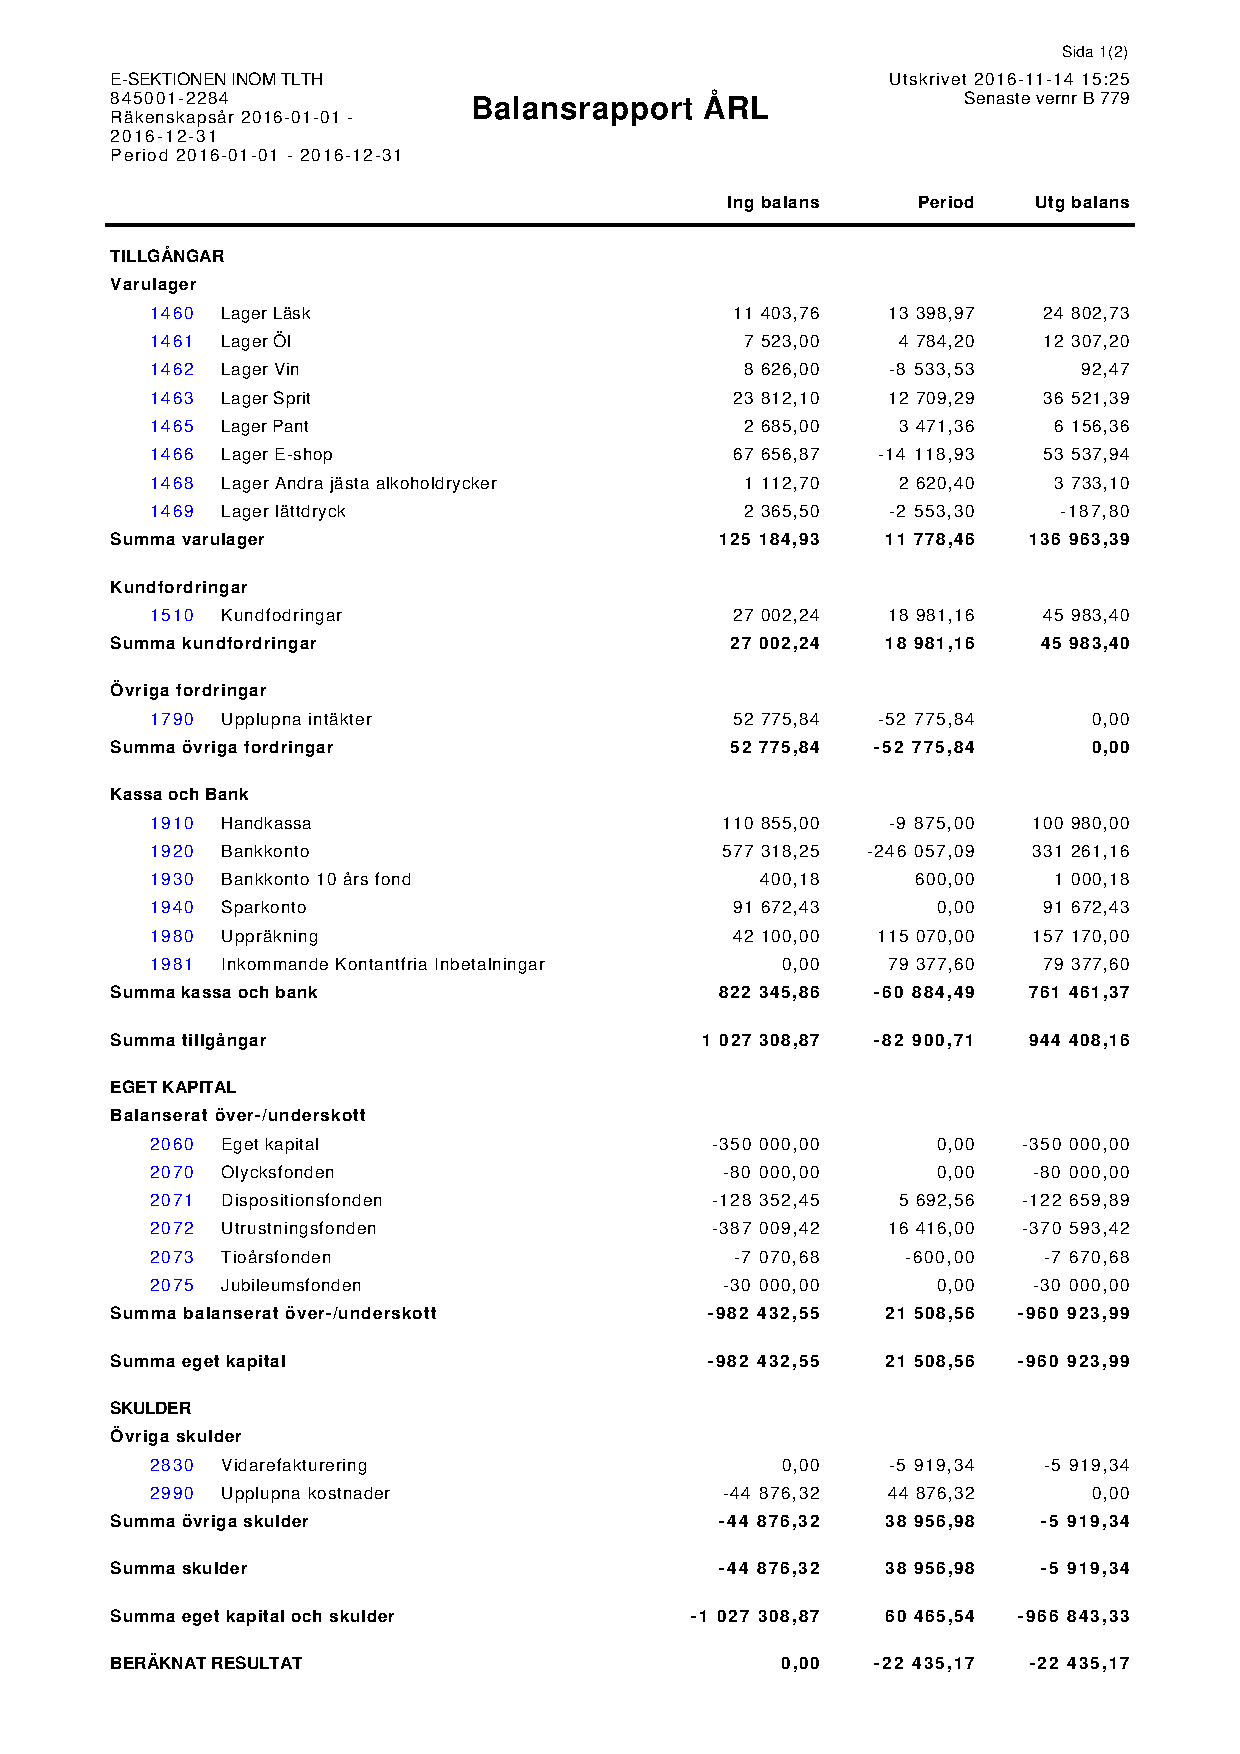
\includepdf[pages=1]{../_res/balansrapport.pdf}

\subfile{../_other/uttag}
\newpage

\begin{supersection}{Beslutsuppföljningar}{}
    \subsection{Överblick}
    \begin{busek}
        \beslutsek{HT/15}{Upprustning av E-husets yttre fasadskylt}{Fredrik Peterson}{Införskaffa ny fasadskylt till en kostnad av maximalt 10 000 kr}{HT/16}
        \beslutsek{VT/16}{Inköp av backuplösning till Sektionens servrar}{Daniel Johansson\newline Andreas Sirenius}{Införskaffa en backuplösning till en kostnad av maximalt 5 500 kr}{HT/16}
        \beslutsek{VT/16}{Inköp av ny spisfläkt till Edekvataköket}{Styrelsen 2016}{Införskaffa en ny fläkt till Edekvataköket till en kostnad av maximalt 22 000 kr inklusive installation}{HT/16}
        \beslutsek{VT/16}{Renovering och ombyggnad av HK och BD}{Styrelsen 2016}{Rusta upp HK och BlåDörren och bland annat flytta väggen mellan rummen till en kostnad av maximalt 30 000 kr}{HT/16}
        \beslutsek{VT/16}{Uppfräschning av gamla arkivet}{Styrelsen 2016}{Rusta upp gamla arkivet med bland annat nya inventarier till en kostnad av maximalt 10 000 kr}{HT/16}
        \beslutsek{VT/16}{Uppfräschning av Diplomat}{Styrelsen 2016}{Rusta upp Diplomat genom ommålning och nya inventarier till en kostnad av maximalt 25 000 kr}{HT/16}
    \end{busek}
    \newpage

    \subfile{../besuppf/fasadskylt}
    \subfile{../besuppf/backupserver}
    \subfile{../besuppf/hkbd}
    \subfile{../besuppf/diplomat}
    \subfile{../besuppf/arkivet}
\end{supersection}

\begin{utskottsrapporter}
    \subfile{../utskottsrapporter/cm}
    \subfile{../utskottsrapporter/e6}
    \subfile{../utskottsrapporter/enu}
    \subfile{../utskottsrapporter/fvu}
    \subfile{../utskottsrapporter/infu}
    \subfile{../utskottsrapporter/km}
    \subfile{../utskottsrapporter/noju}
    \subfile{../utskottsrapporter/nollu}
    \subfile{../utskottsrapporter/sre}
    \subfile{../utskottsrapporter/styrelsen}
    \subfile{../utskottsrapporter/vb}
\end{utskottsrapporter}

\begin{supersection}{Verksamhetsplaner}{}
    \subfile{../verksplaner/2016}
\end{supersection}

\begin{supersection}{Uppföljningar av verksamhetsplaner}{}
    \subfile{../verksplanuppfar/2016-vt}
    \subfile{../verksplanuppfar/2016-ht}
\end{supersection}

\begin{motioner}
    \subfile{../motioner/bahamas}
    \subfile{../motionssvar/bahamas}
    \subfile{../motioner/salami}
    \subfile{../motionssvar/salami}
    \subfile{../motioner/qasque}
    \subfile{../motionssvar/qasque}
    \subfile{../motioner/mongo}
    \subfile{../motionssvar/mongo}
    \subfile{../motioner/diskho}
    \subfile{../motionssvar/diskho}
    \subfile{../motioner/fanan}
    \subfile{../motionssvar/fanan}
\end{motioner}

\begin{propositioner}
    \subfile{../propositioner/_budget}
    \subfile{../propositioner/_verkplan}
    \subfile{../propositioner/ta_bort_jaml_policy}
    \subfile{../propositioner/klader}
    \subfile{../propositioner/alkohol}
    \subfile{../propositioner/medalj}
    \subfile{../propositioner/overvakning}
    \subfile{../propositioner/kompletterande_sre}
    \subfile{../propositioner/beskr}
    \subfile{../propositioner/antal_fvu}
    \subfile{../propositioner/antal_cm}
    \subfile{../propositioner/antal}
    \subfile{../propositioner/switch}
    \subfile{../propositioner/datorer}
\end{propositioner}

\begin{supersection}{Halvårsbokslut 2016}{}
    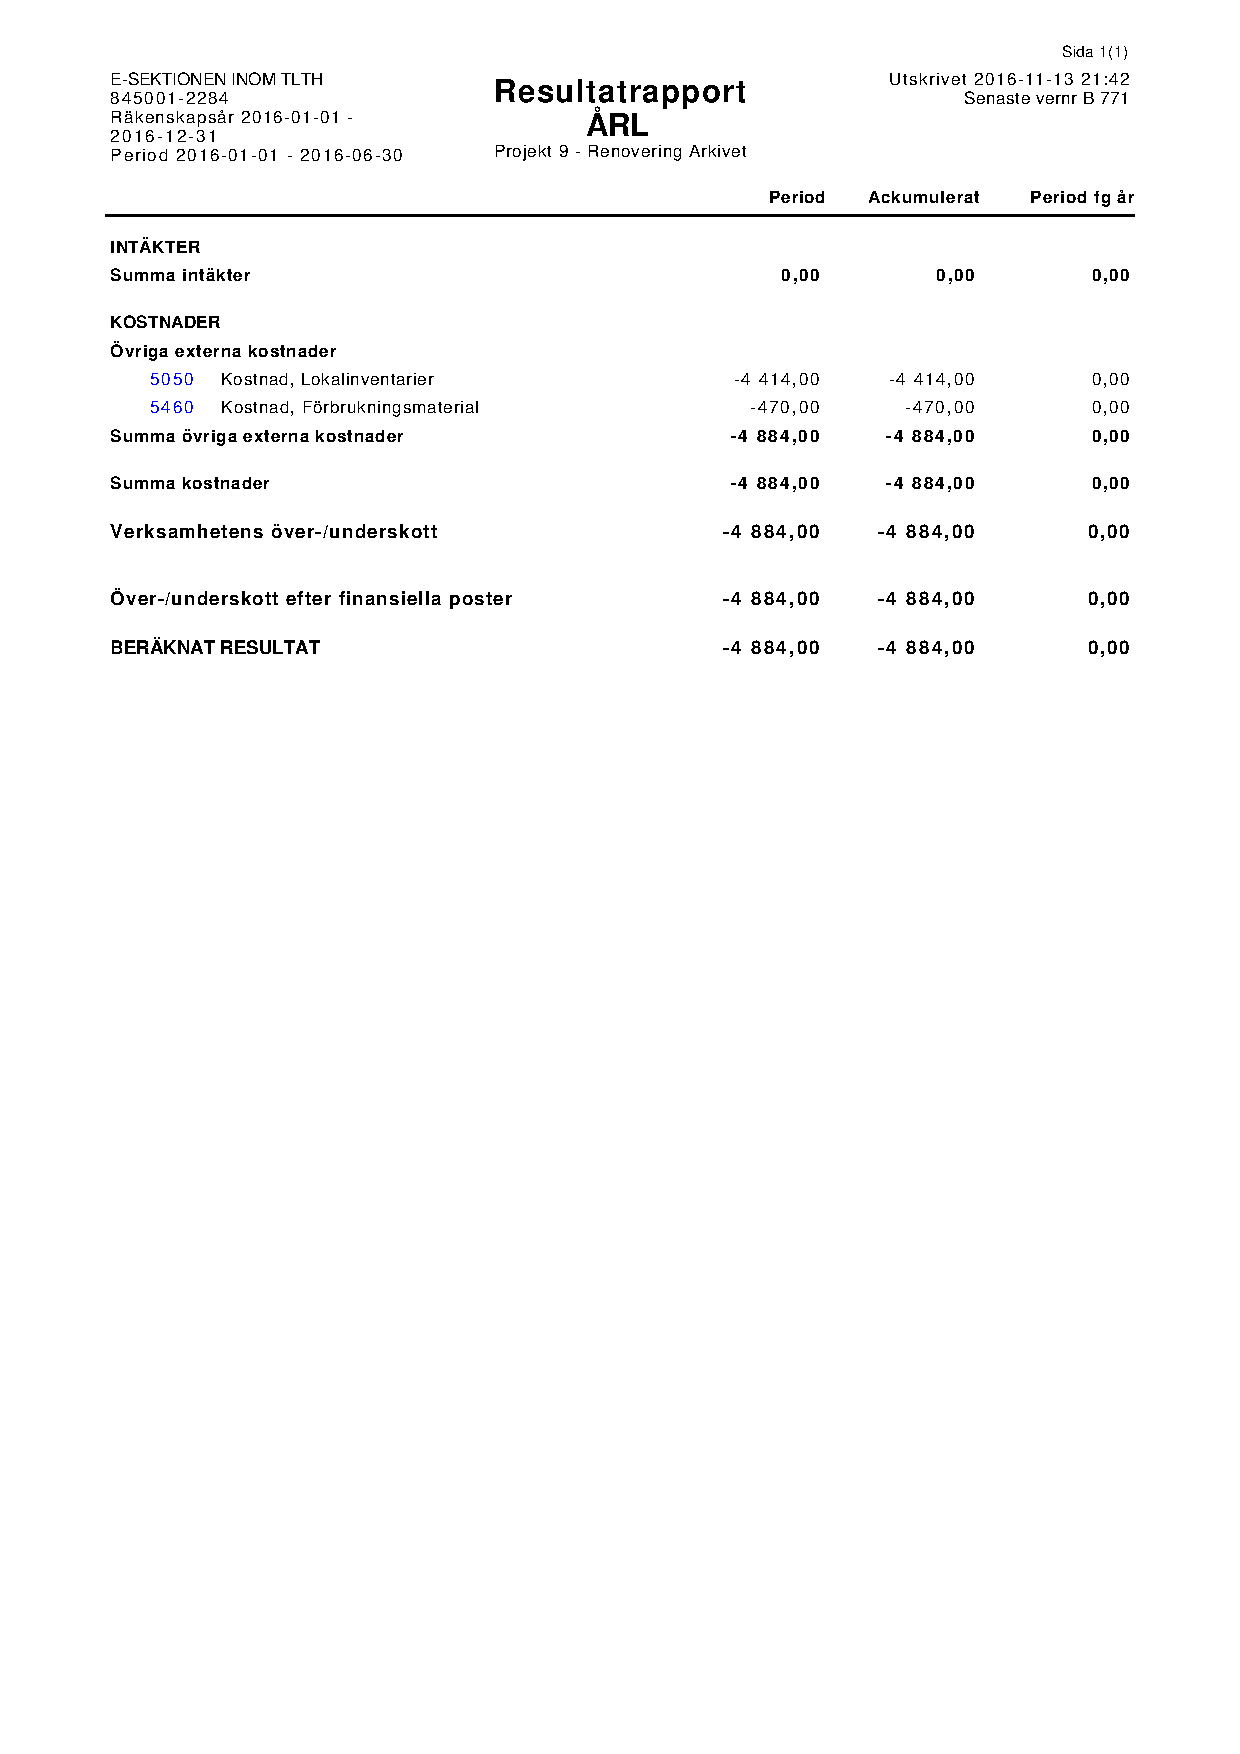
\includepdf[pages=-]{../_res/bokslut/arkivet.pdf}
    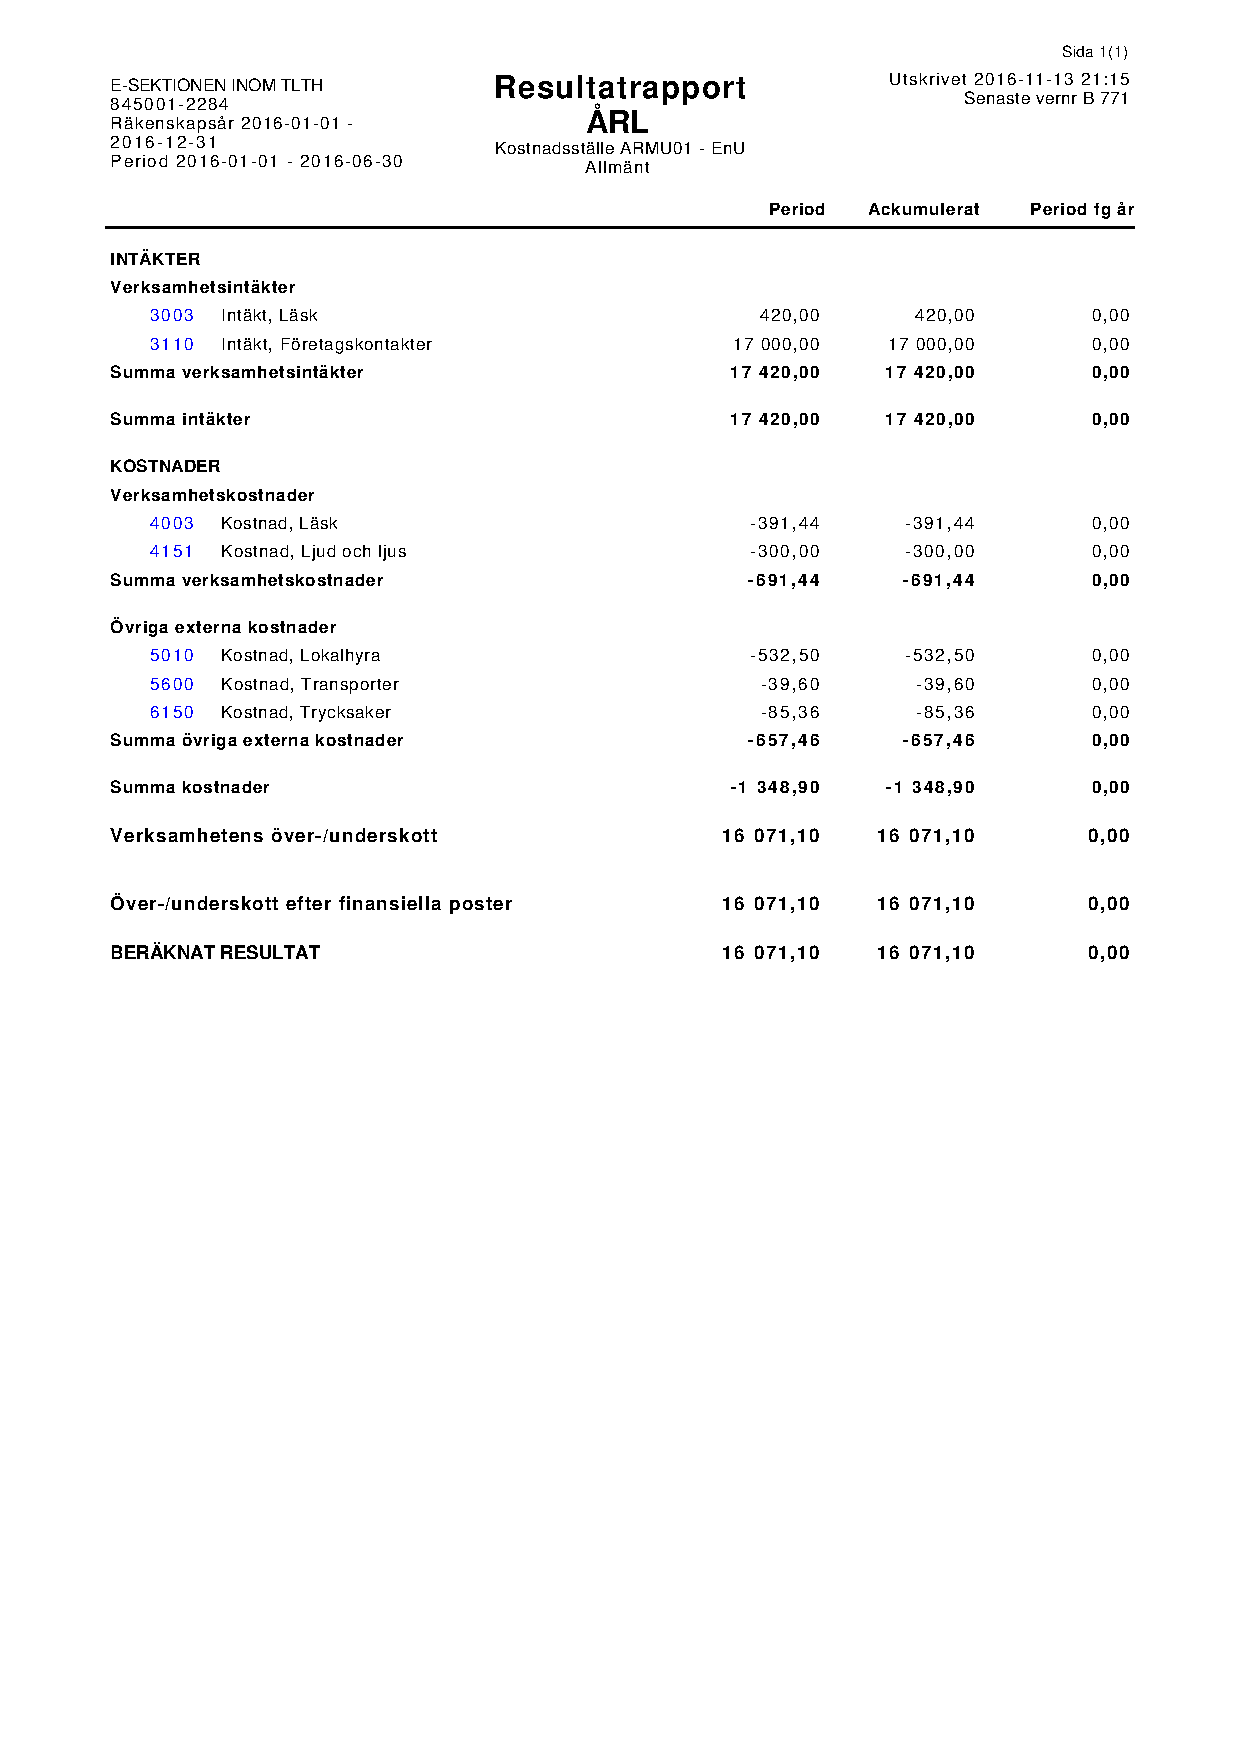
\includepdf[pages=-]{../_res/bokslut/armu01.pdf}
    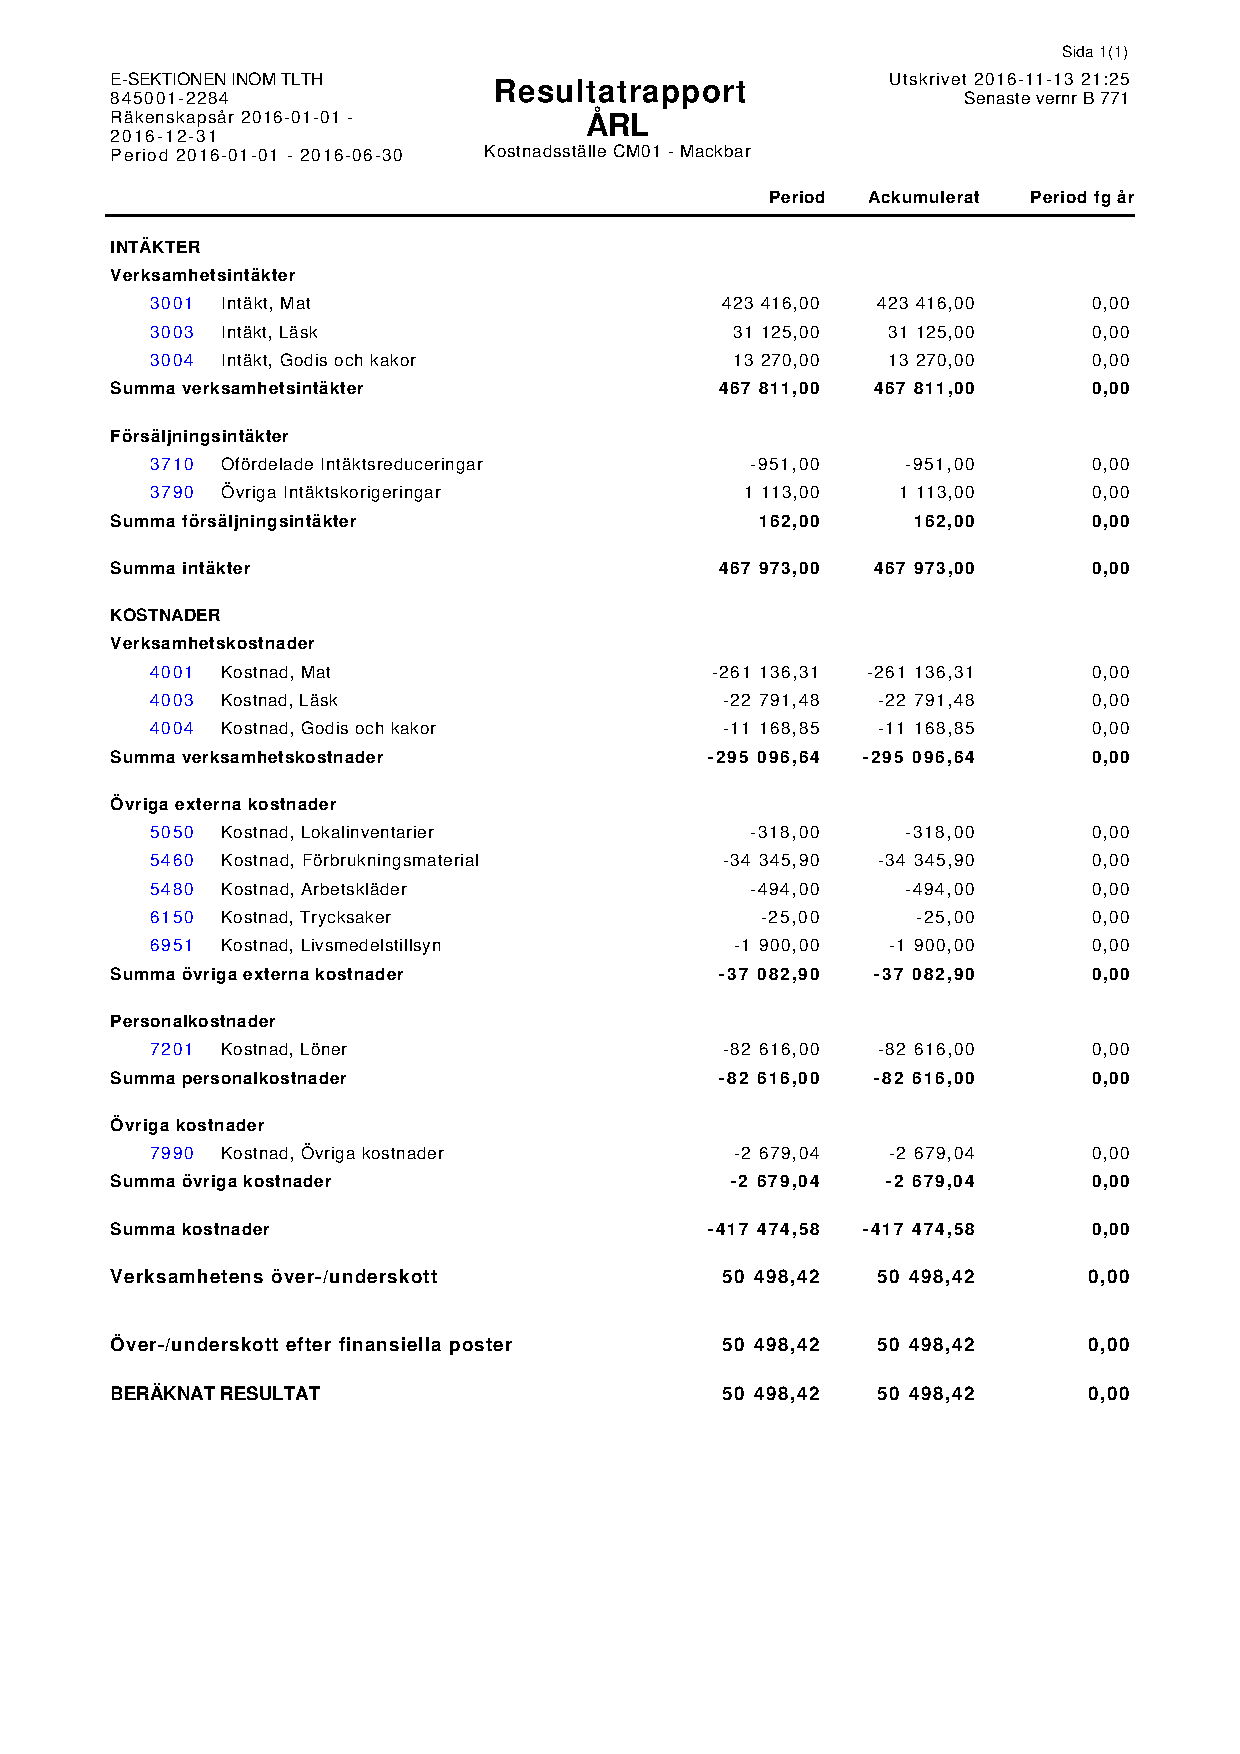
\includepdf[pages=-]{../_res/bokslut/cm01.pdf}
    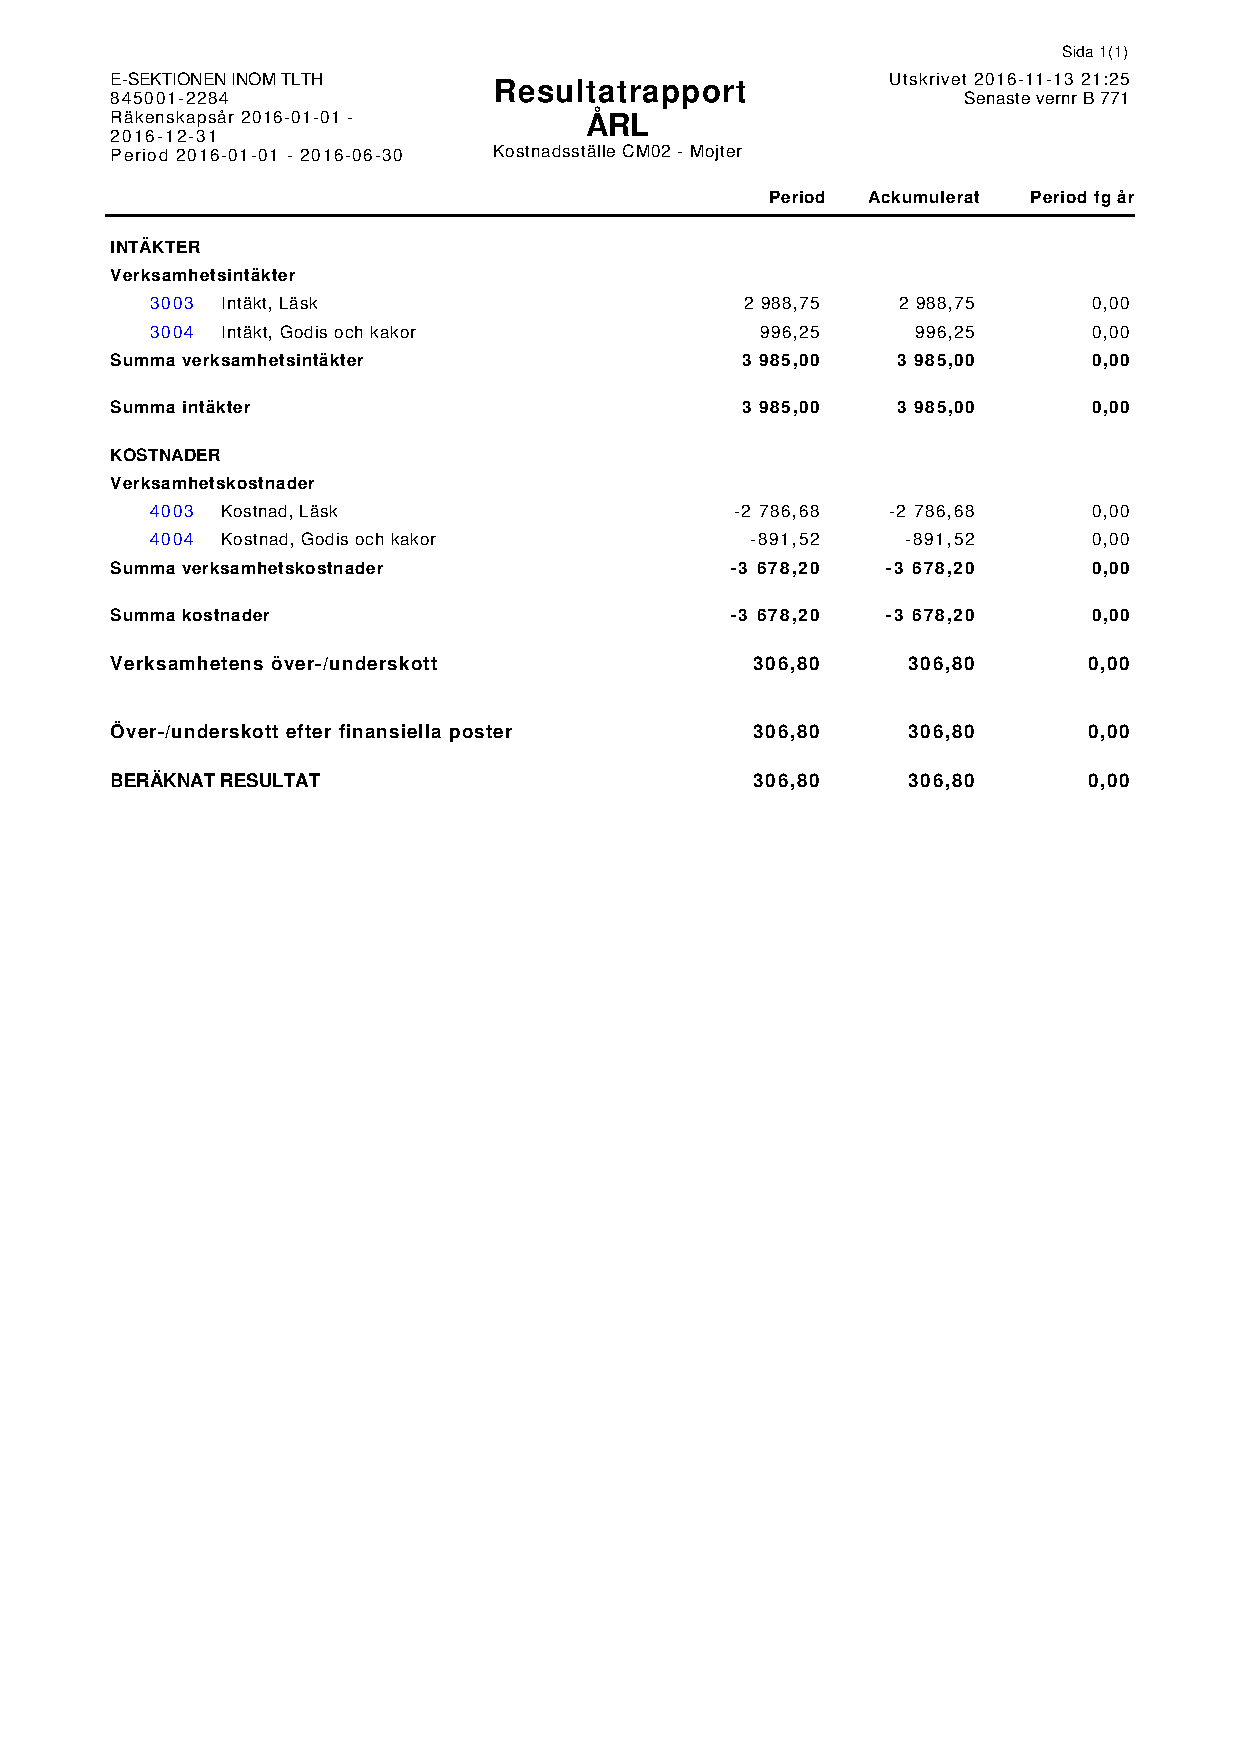
\includepdf[pages=-]{../_res/bokslut/cm02.pdf}
    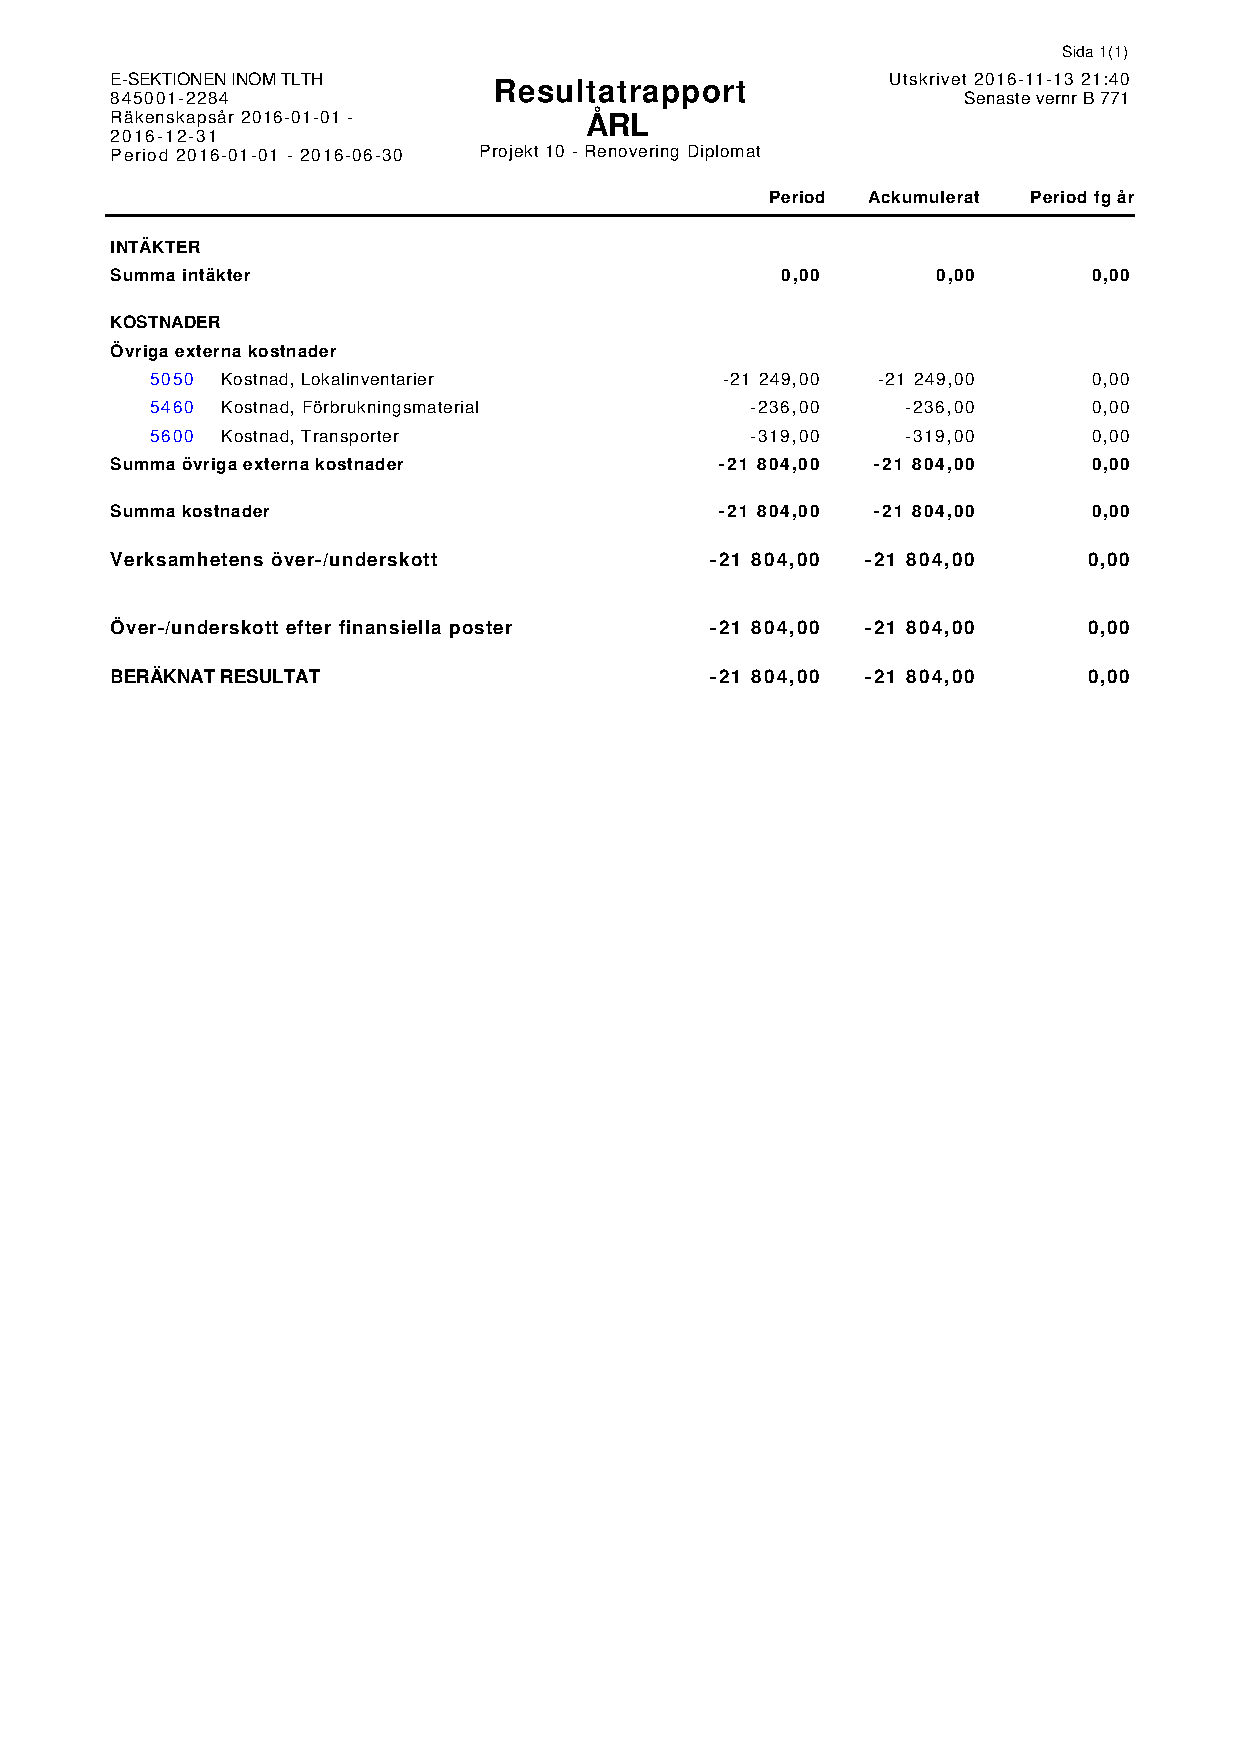
\includepdf[pages=-]{../_res/bokslut/diplomat.pdf}
    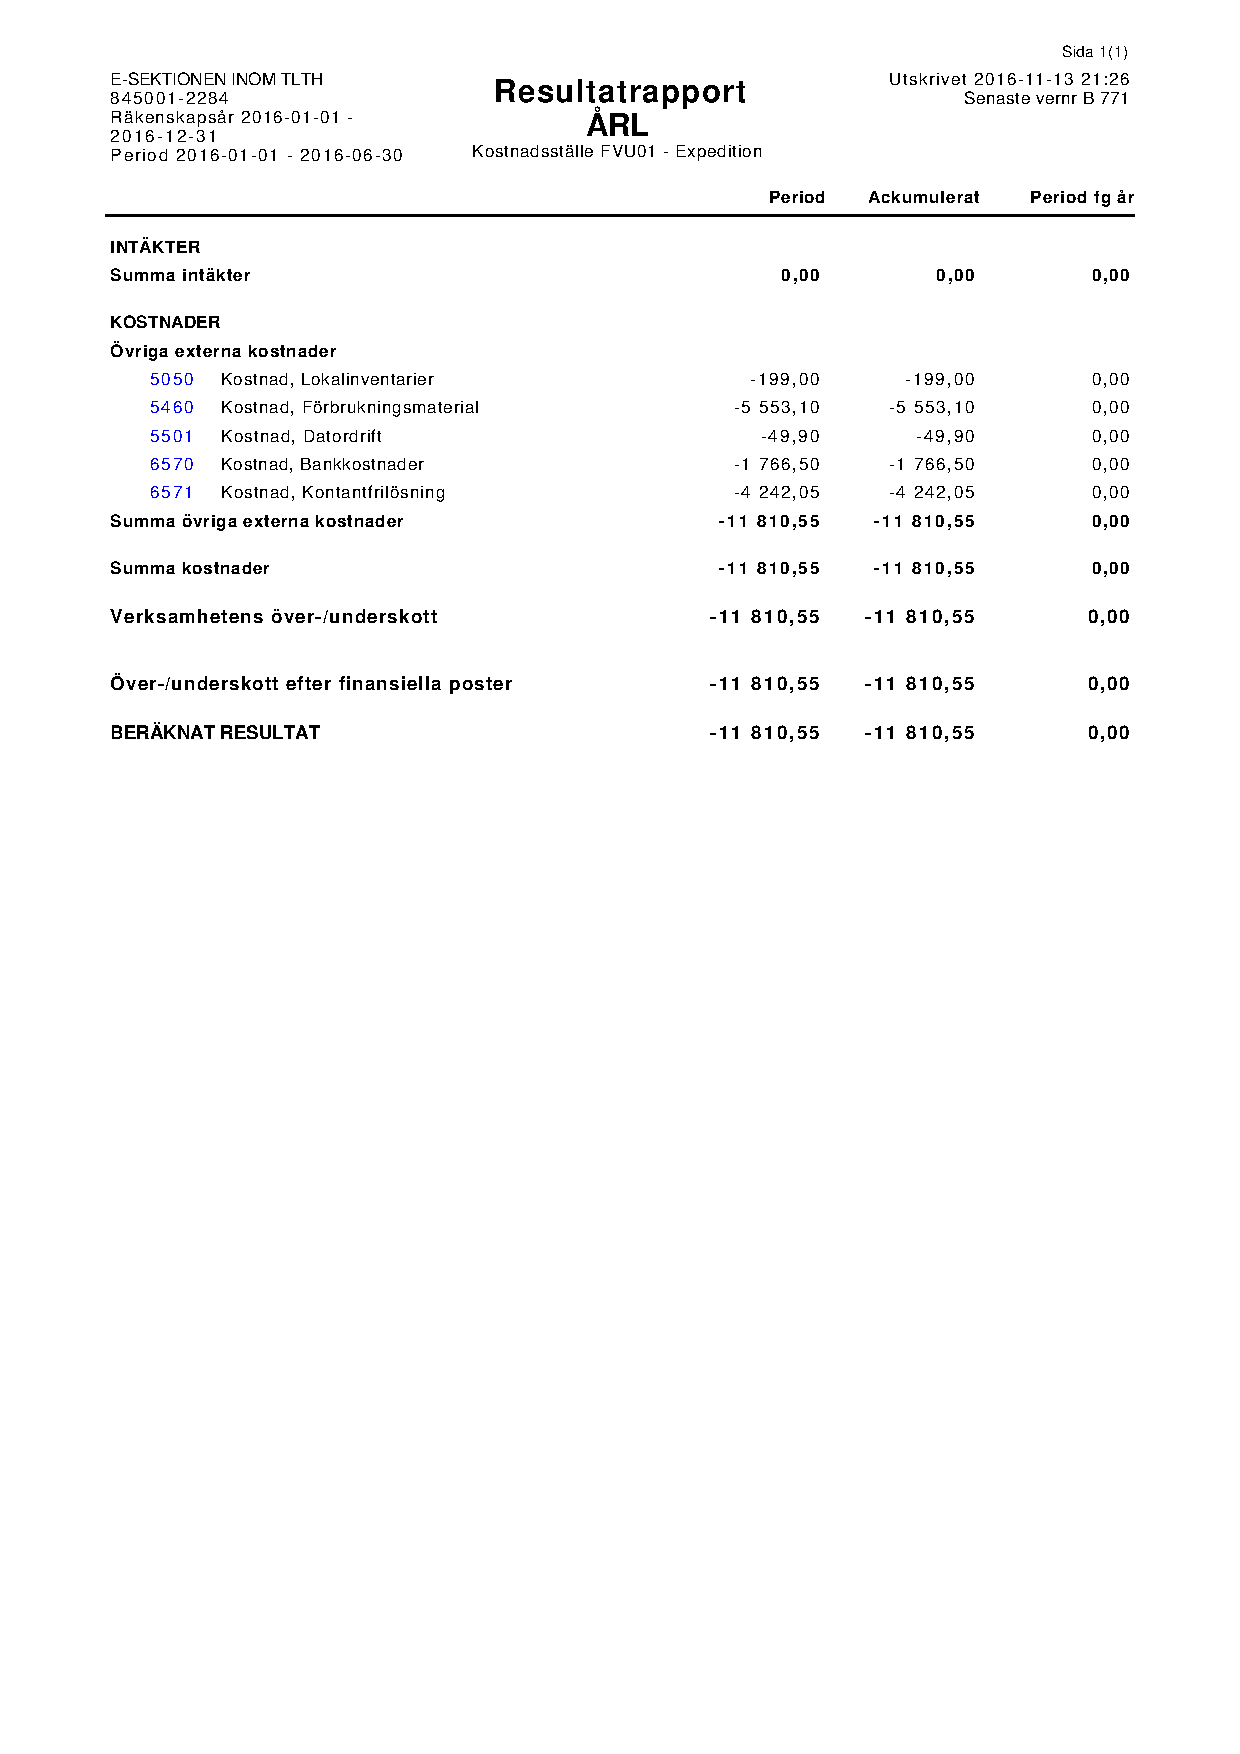
\includepdf[pages=-]{../_res/bokslut/fvu01.pdf}
    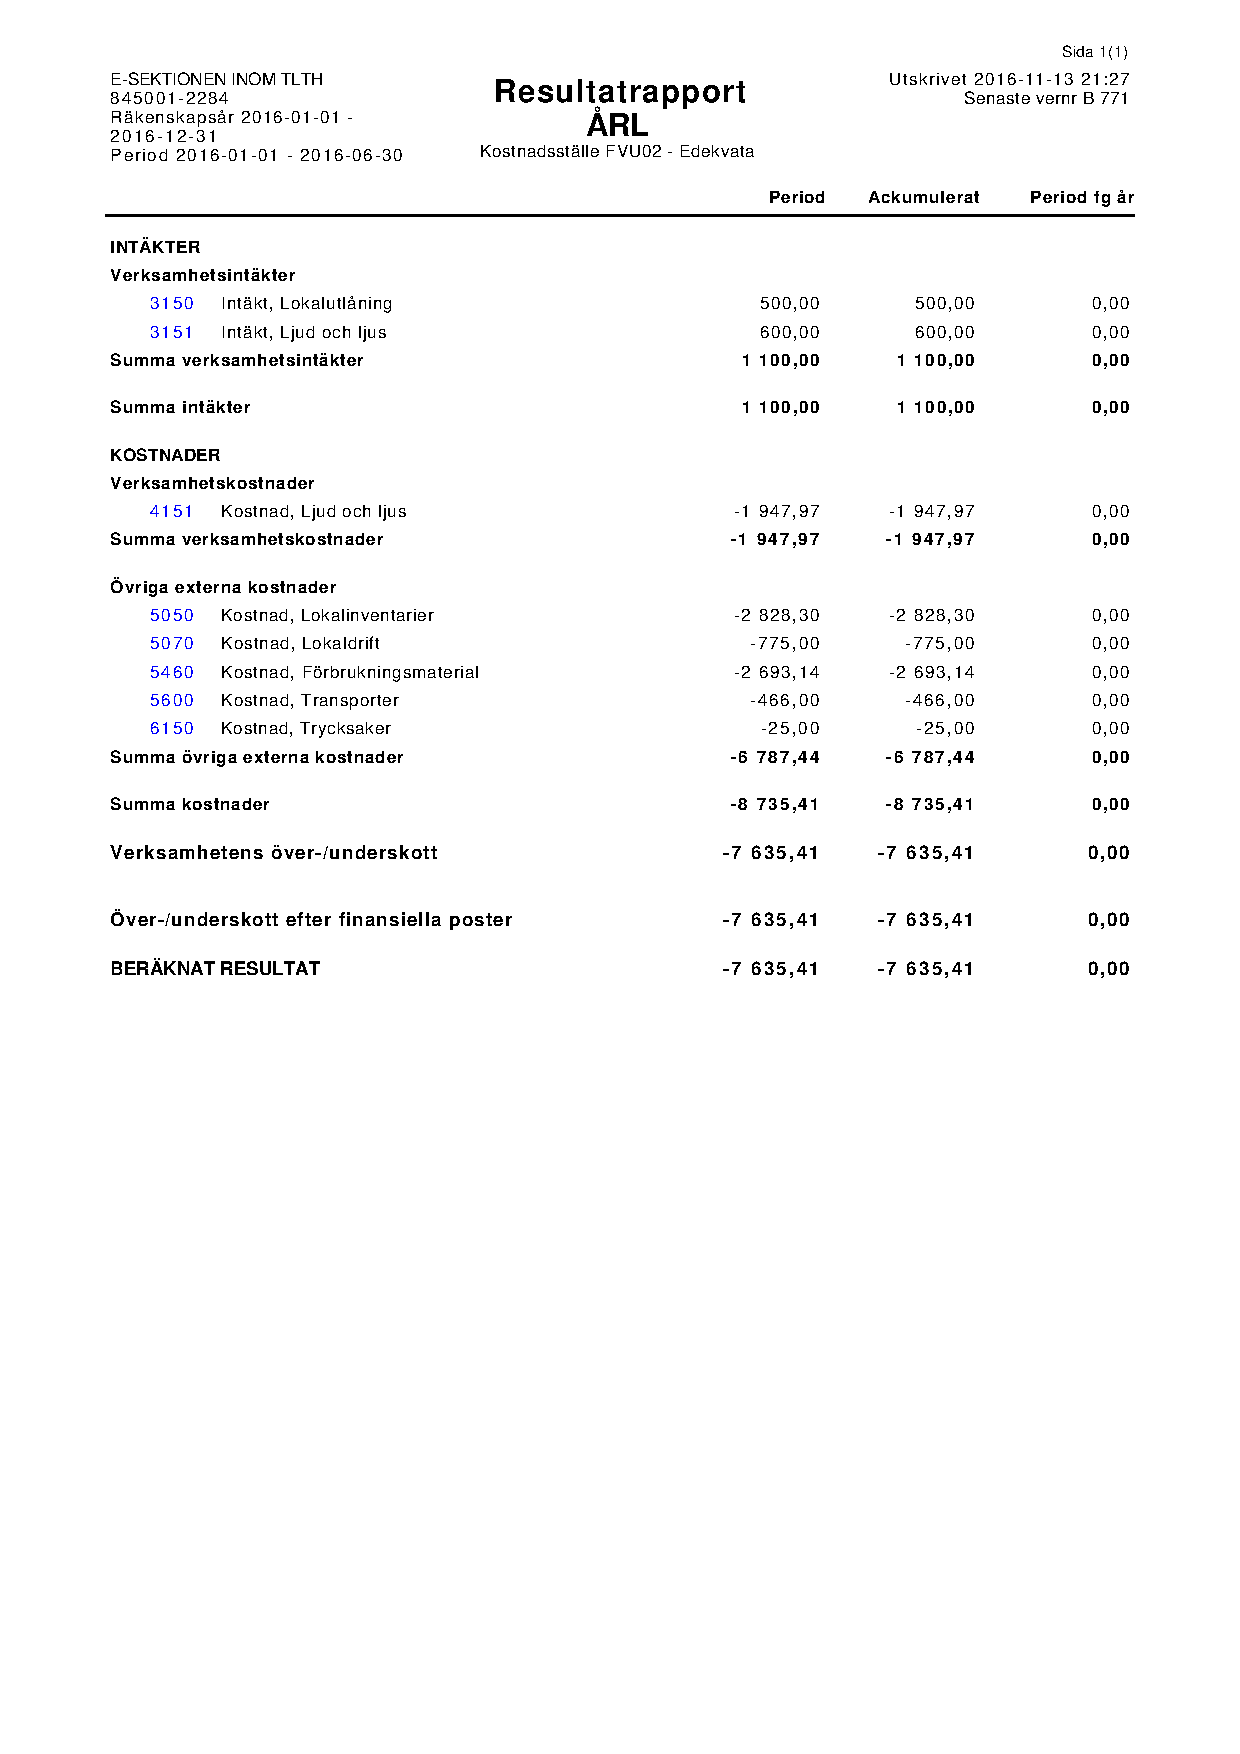
\includepdf[pages=-]{../_res/bokslut/fvu02.pdf}
    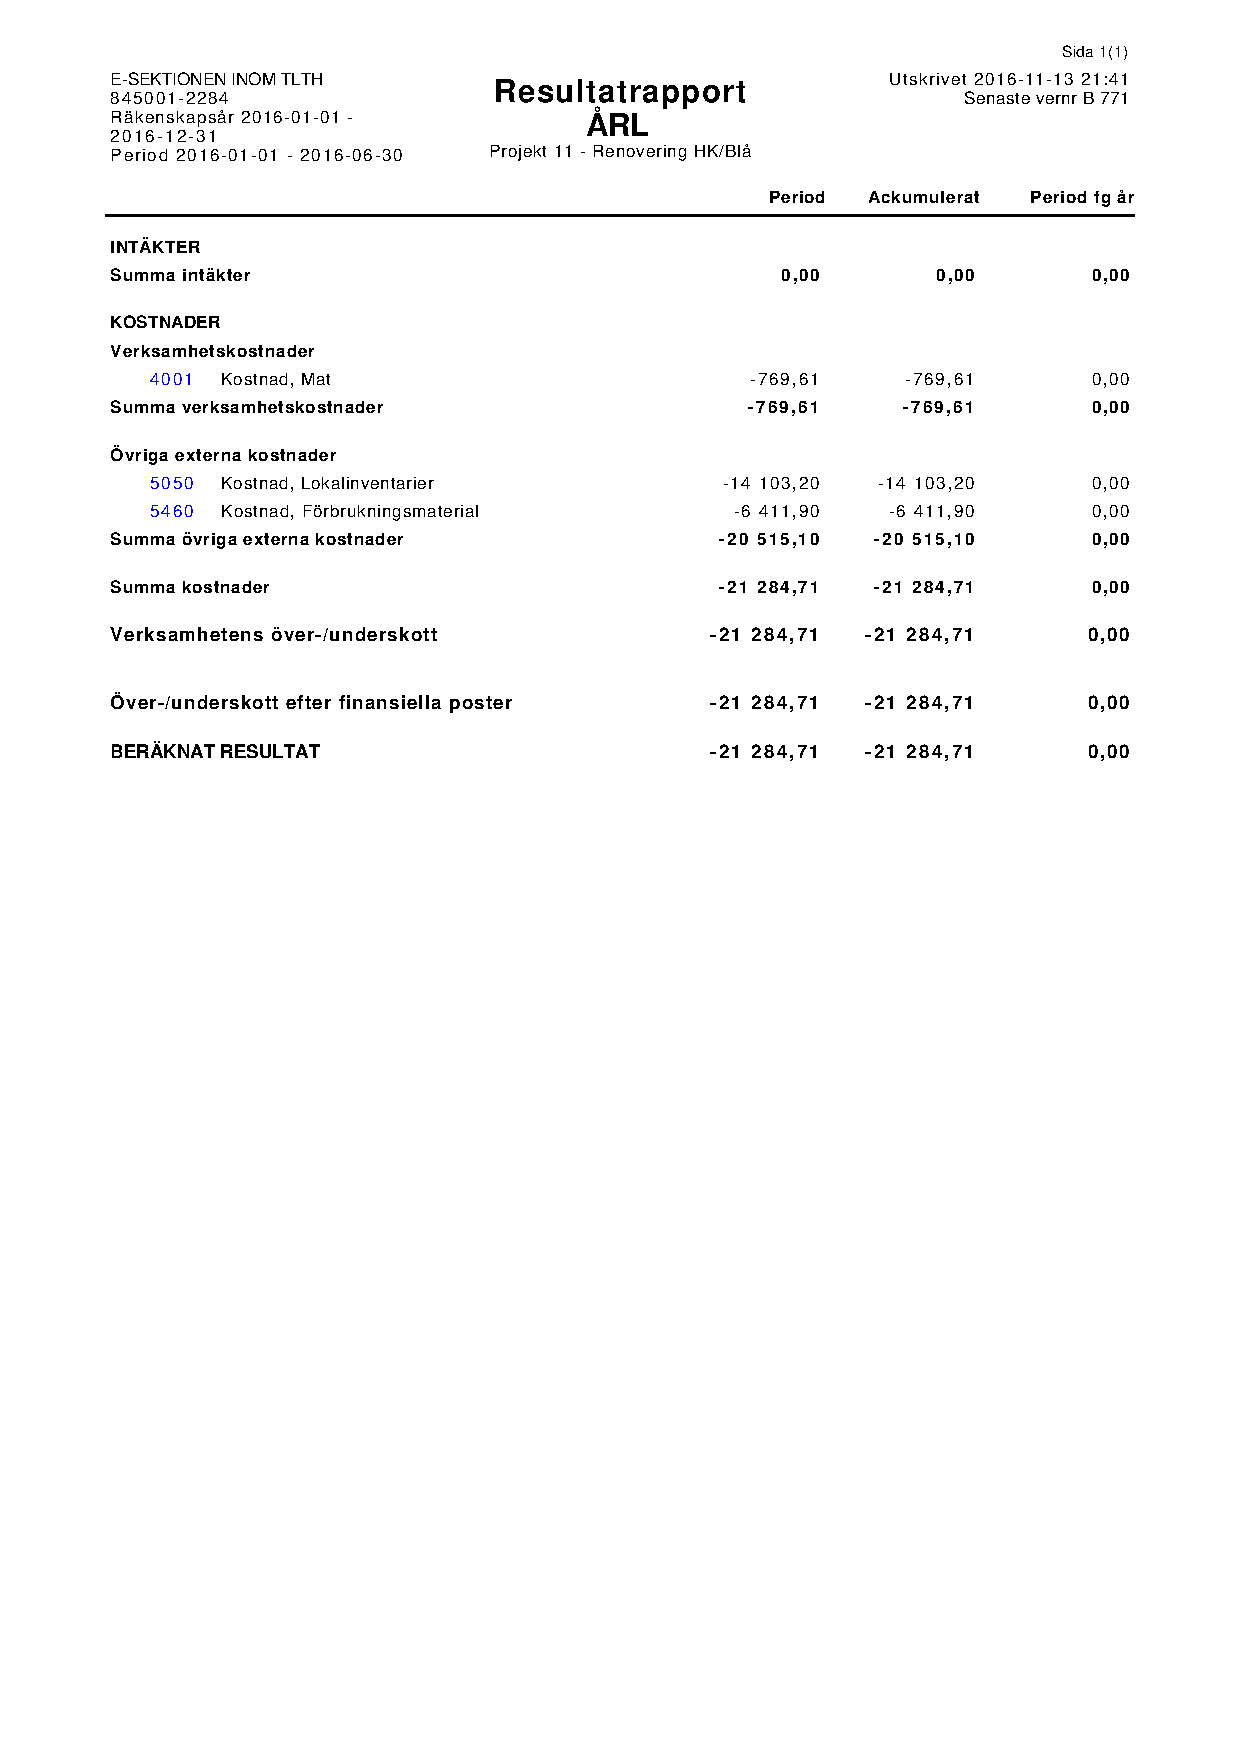
\includepdf[pages=-]{../_res/bokslut/hk.pdf}
    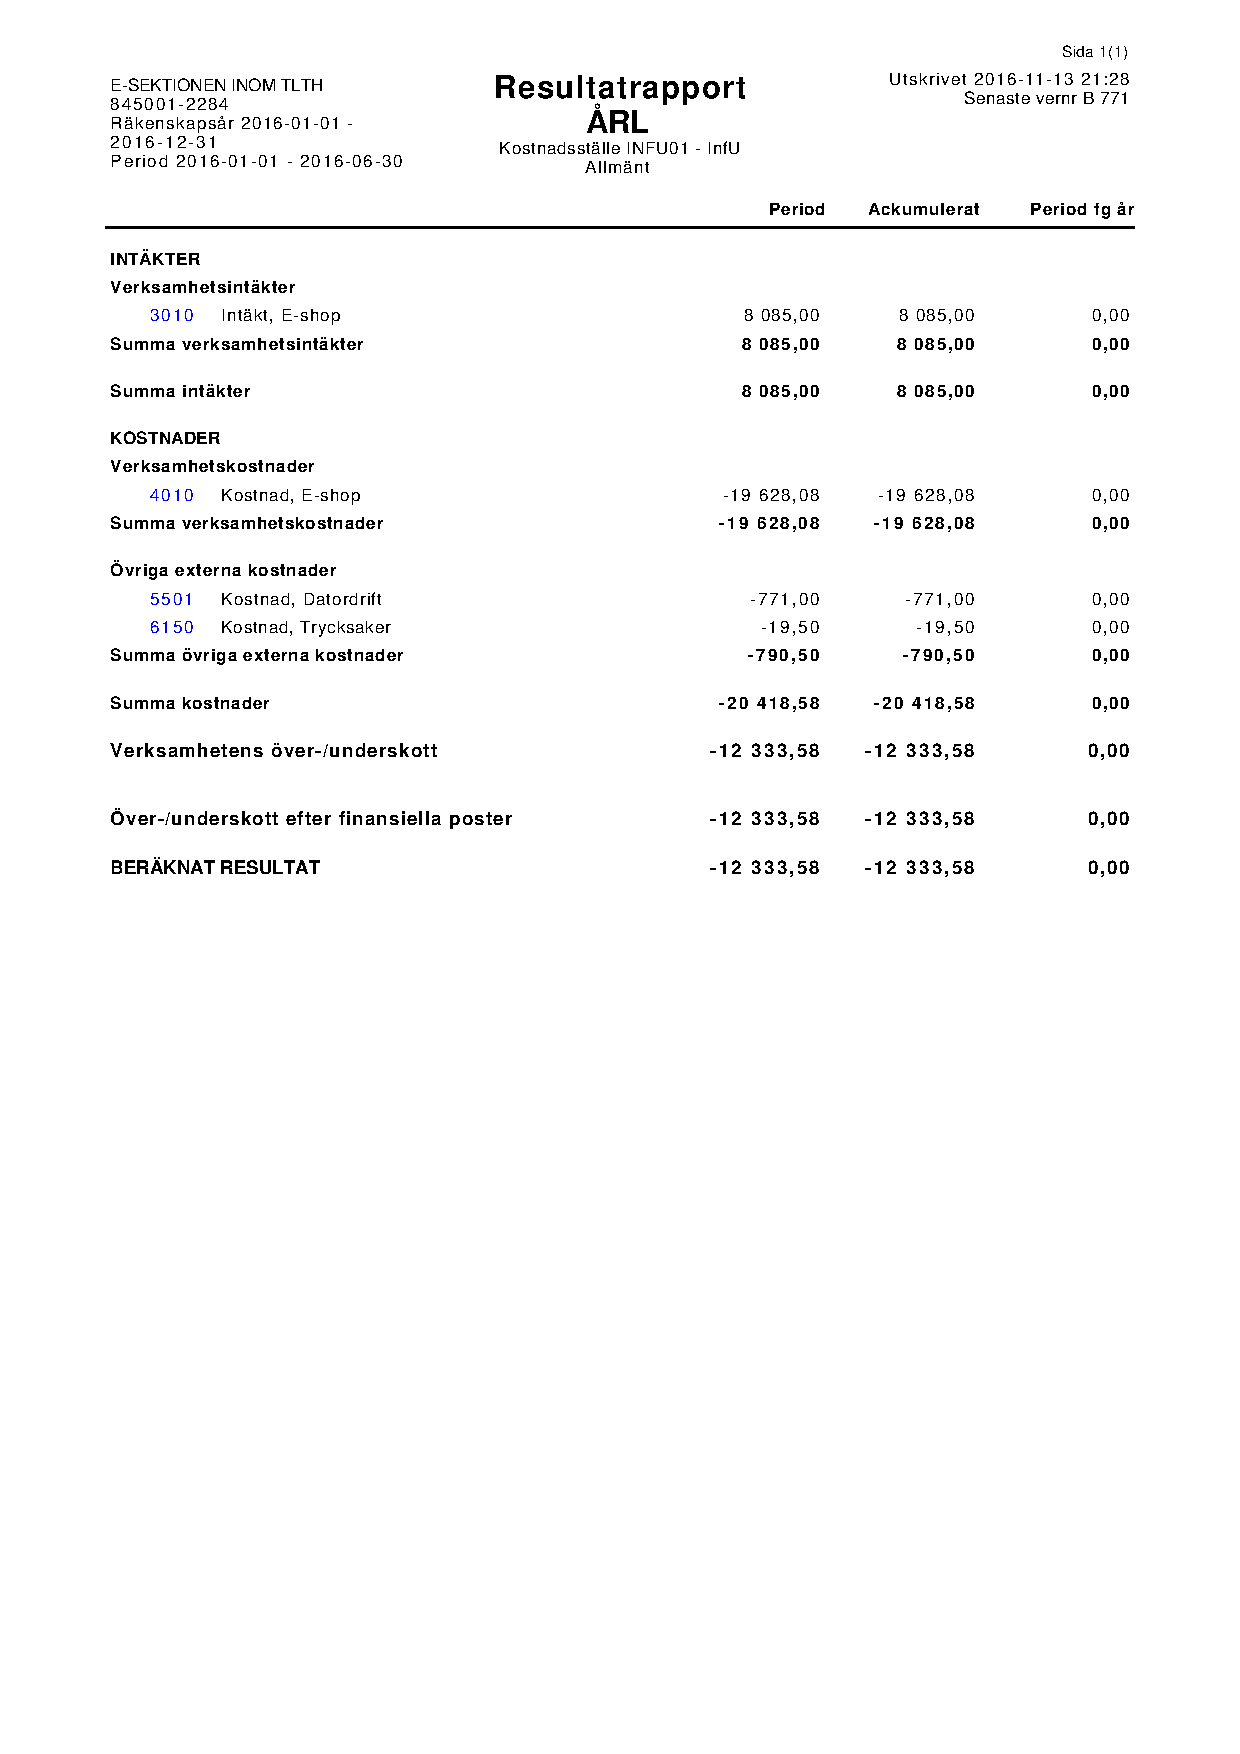
\includepdf[pages=-]{../_res/bokslut/infu01.pdf}
    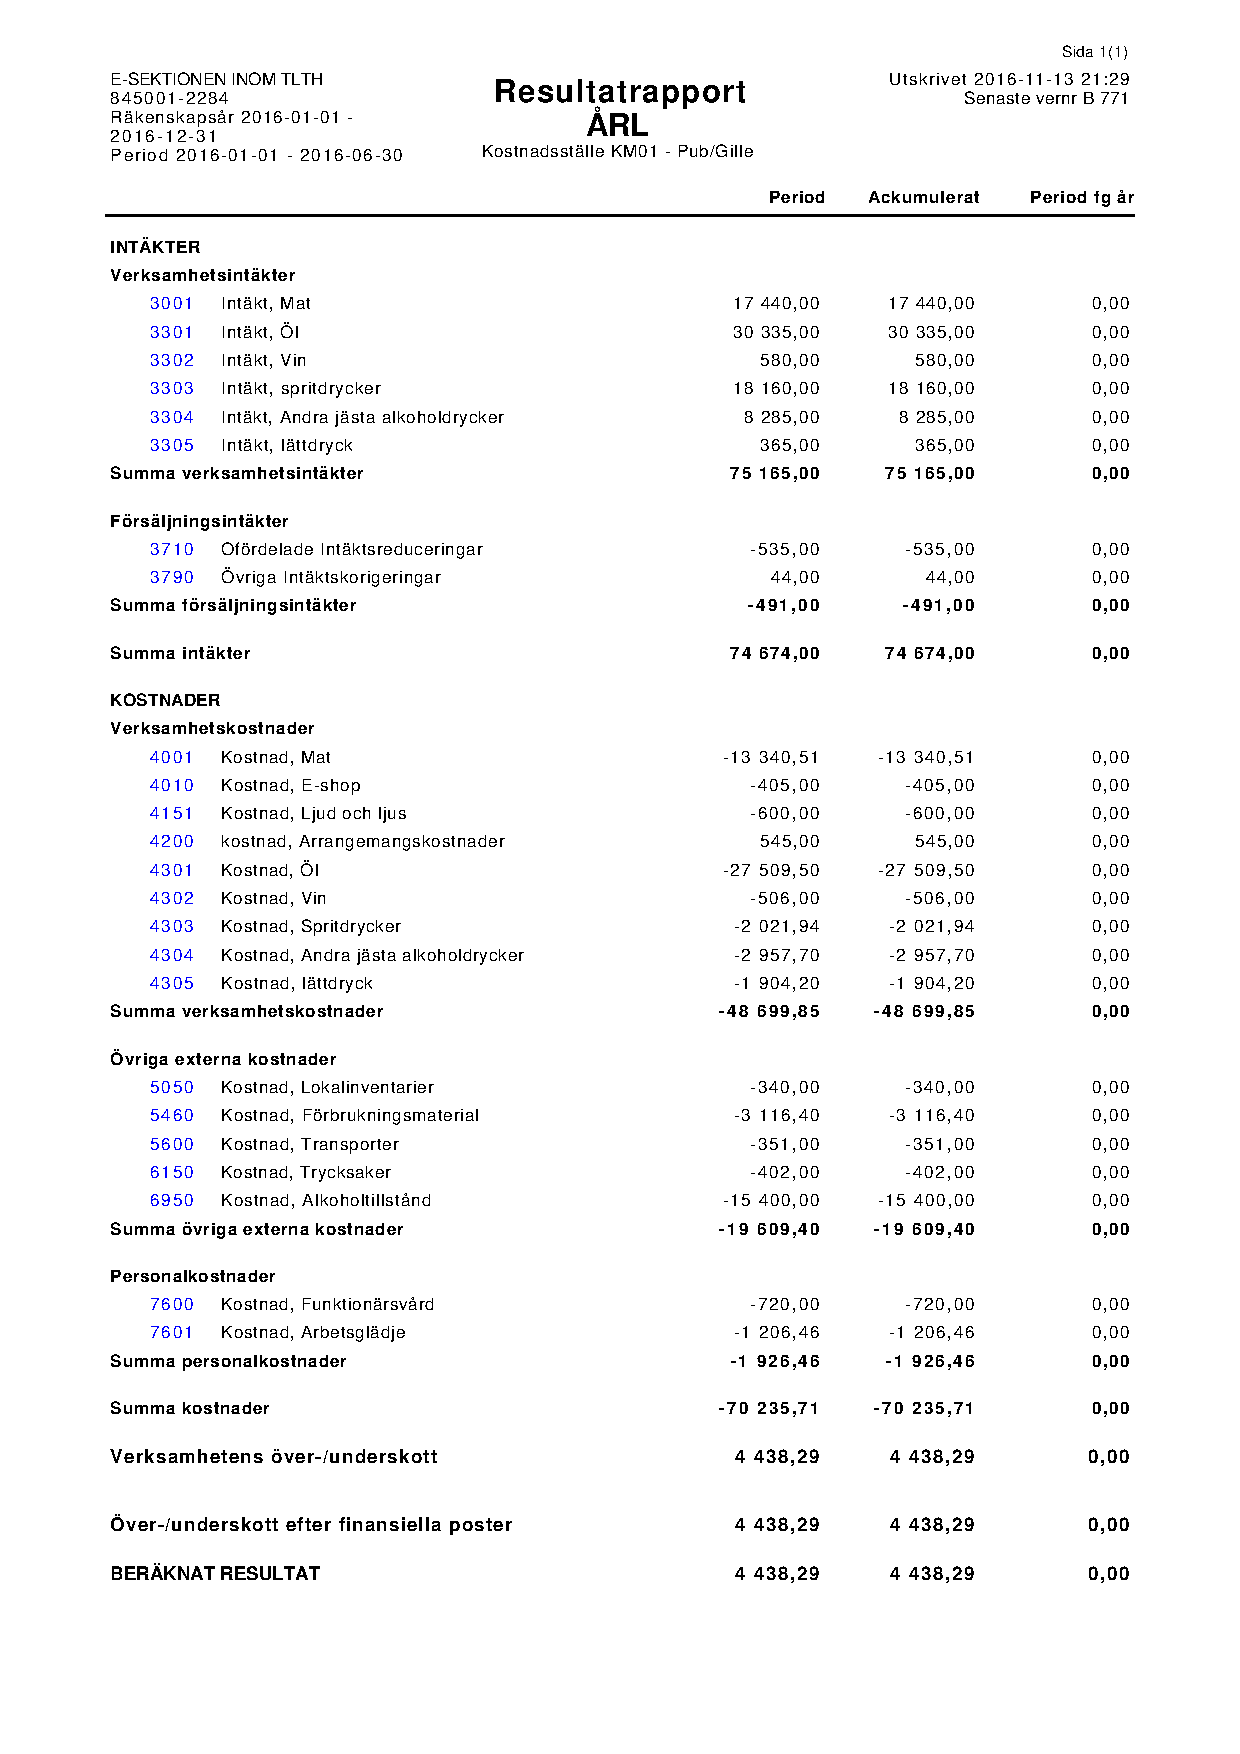
\includepdf[pages=-]{../_res/bokslut/km01.pdf}
    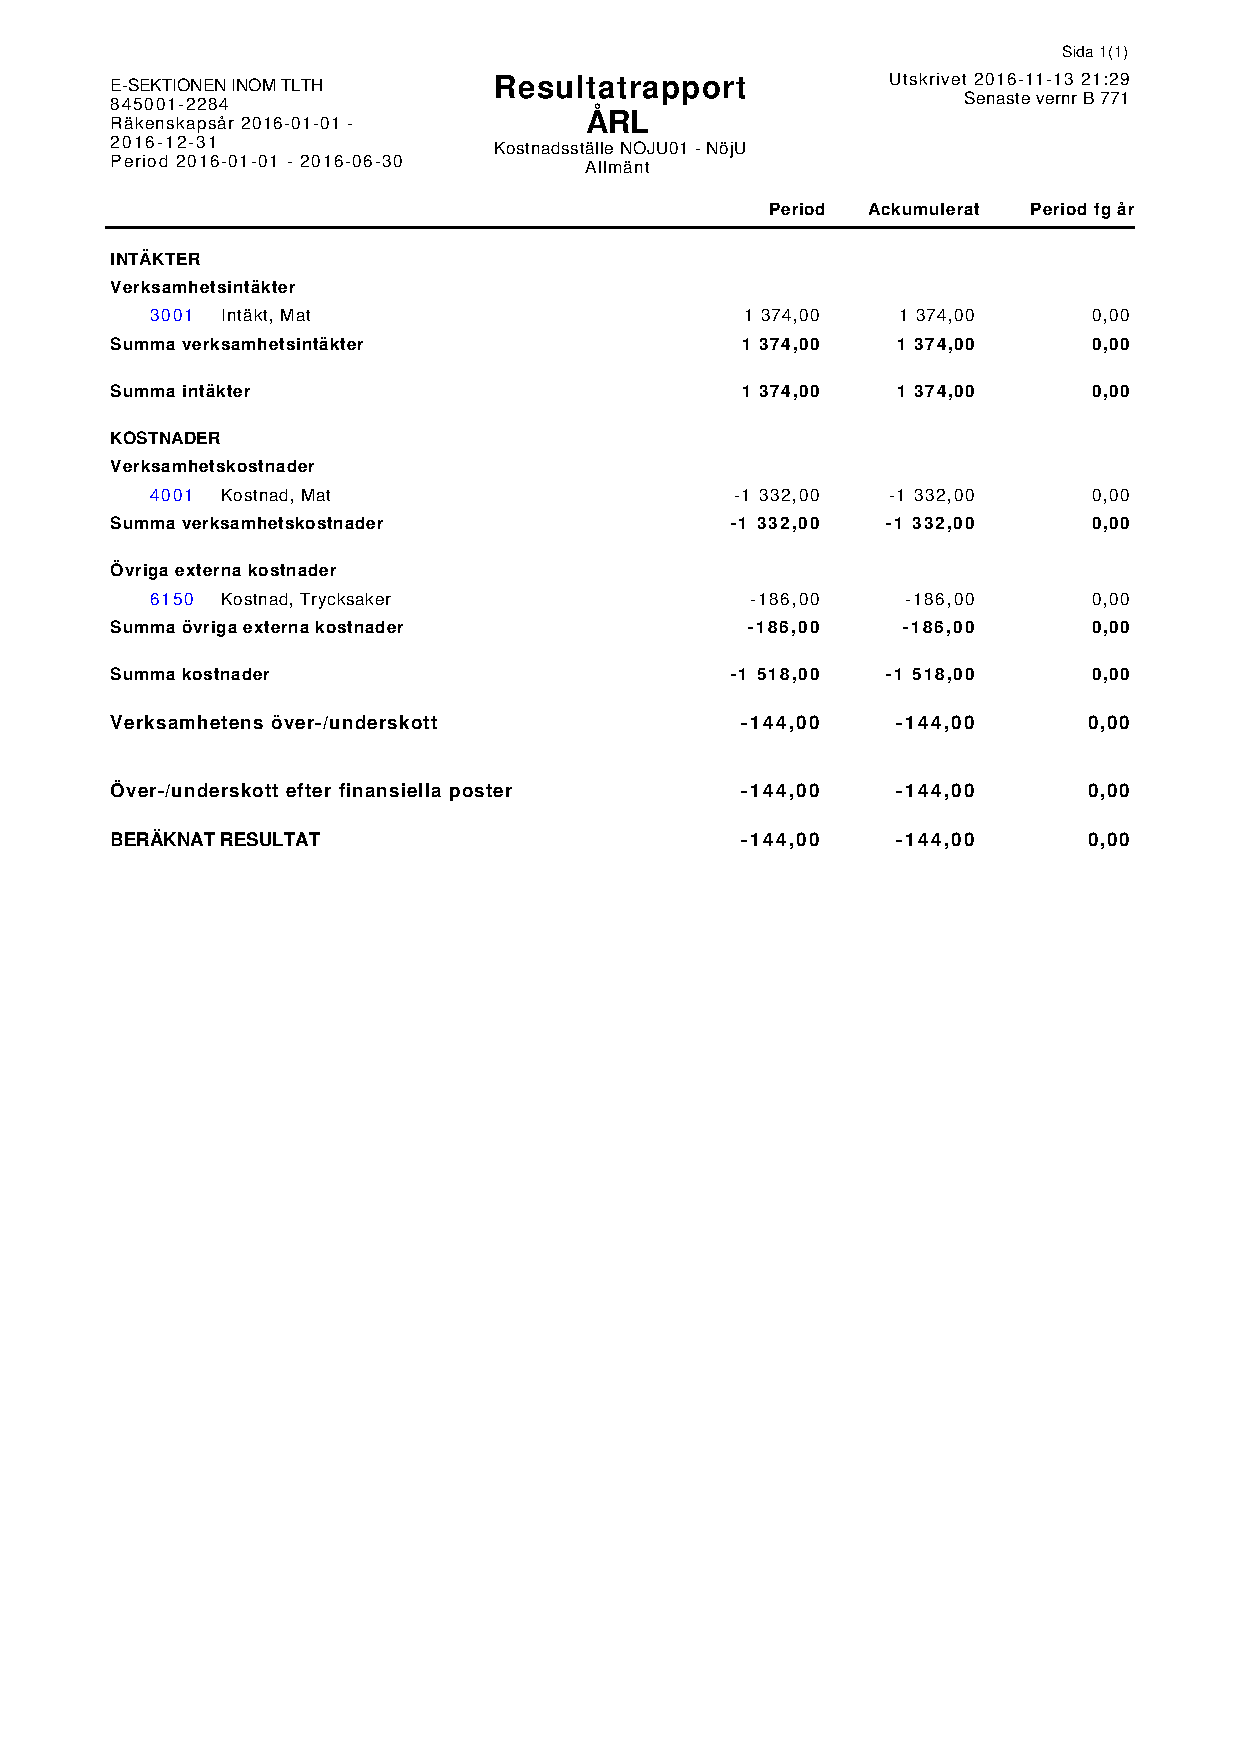
\includepdf[pages=-]{../_res/bokslut/noju01.pdf}
    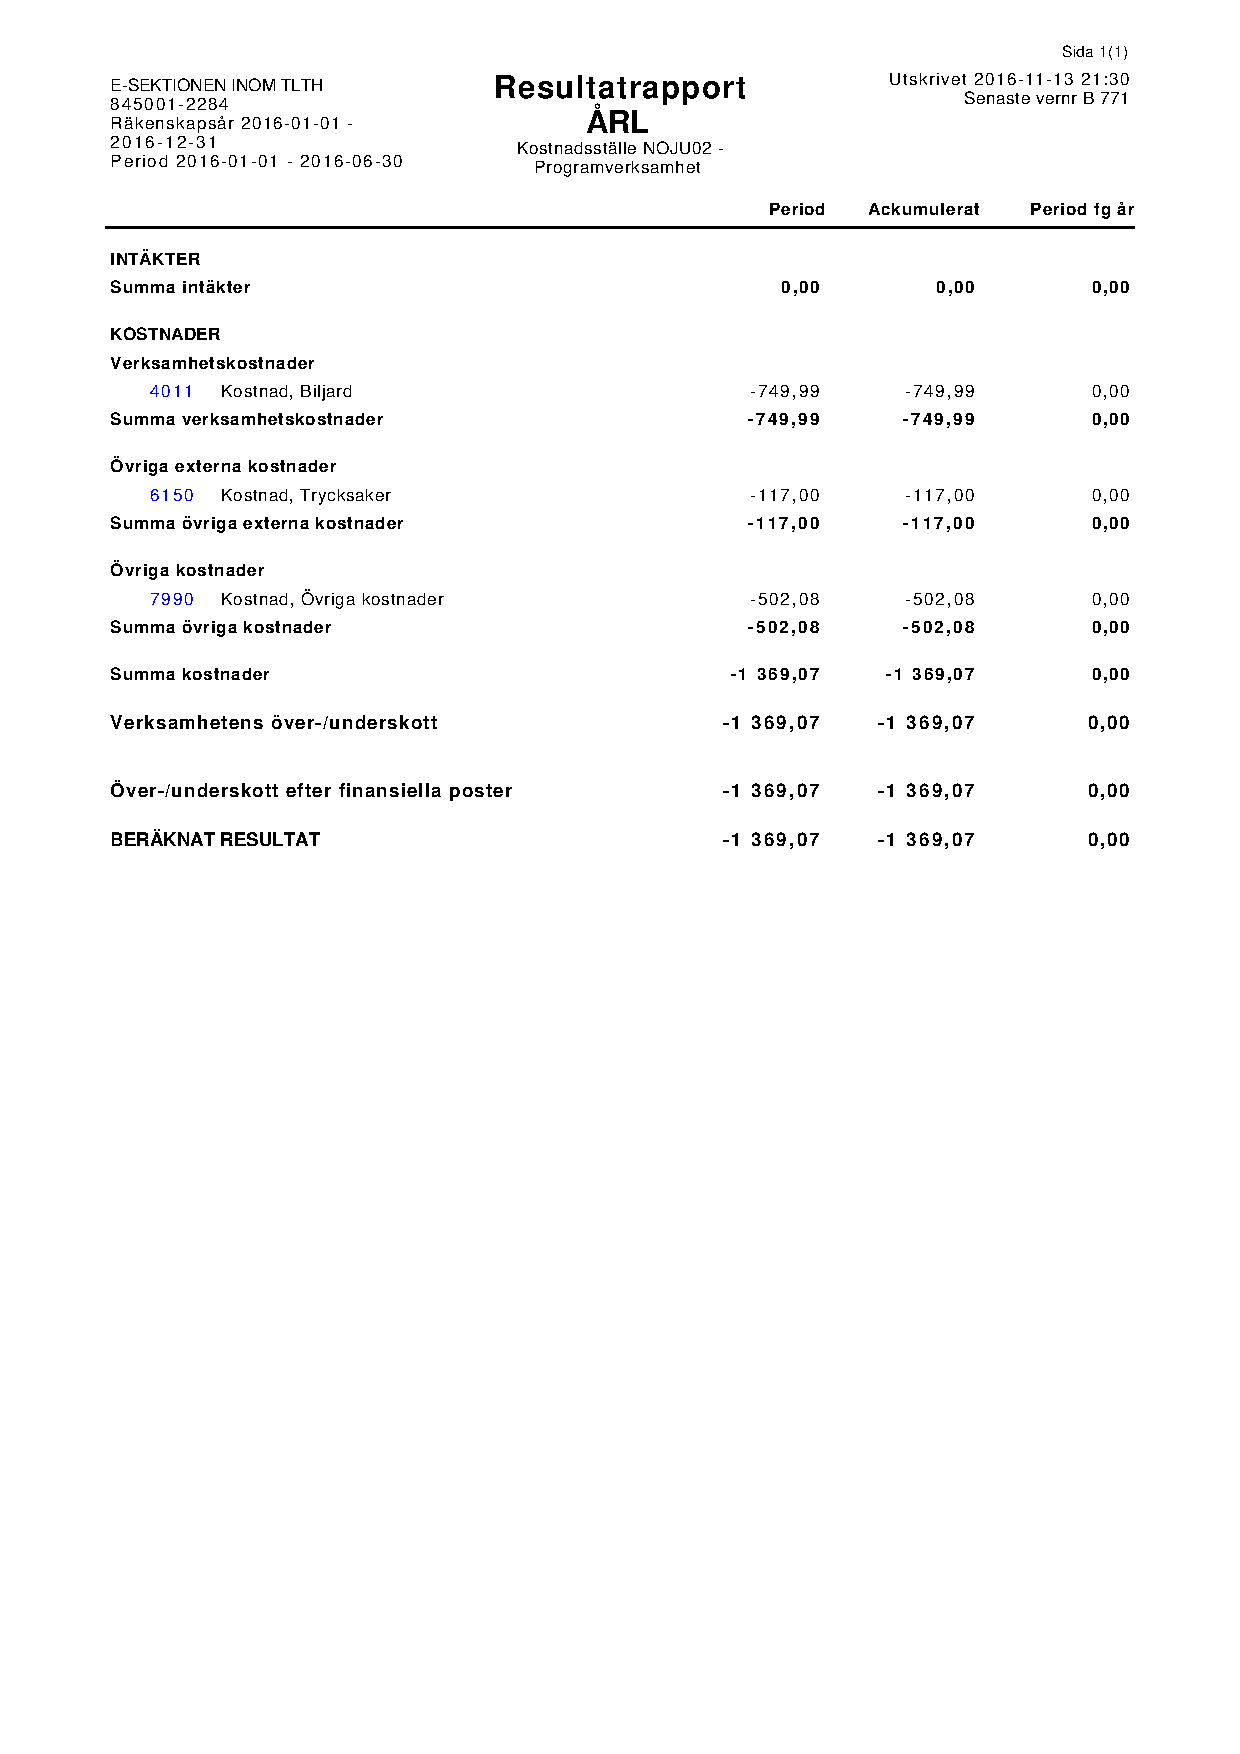
\includepdf[pages=-]{../_res/bokslut/noju02.pdf}
    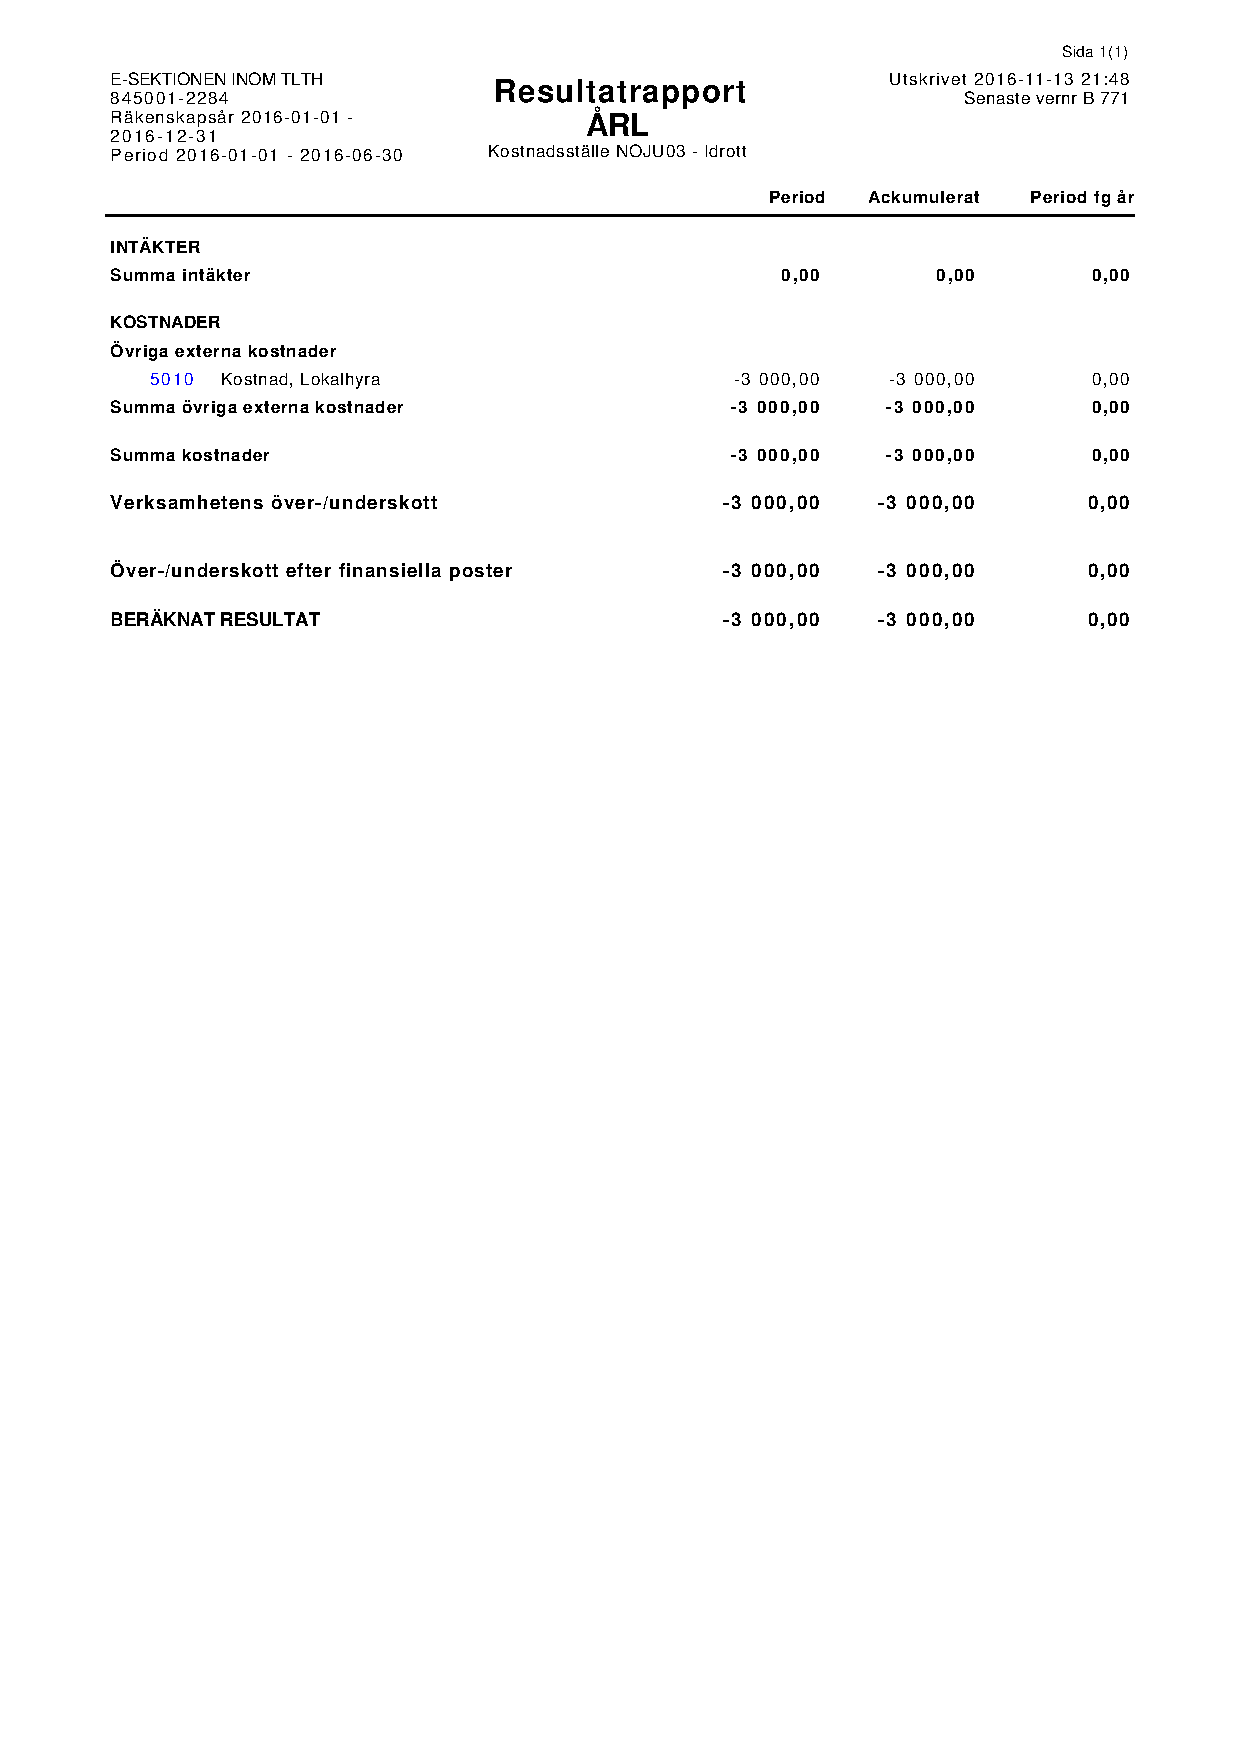
\includepdf[pages=-]{../_res/bokslut/noju03.pdf}
    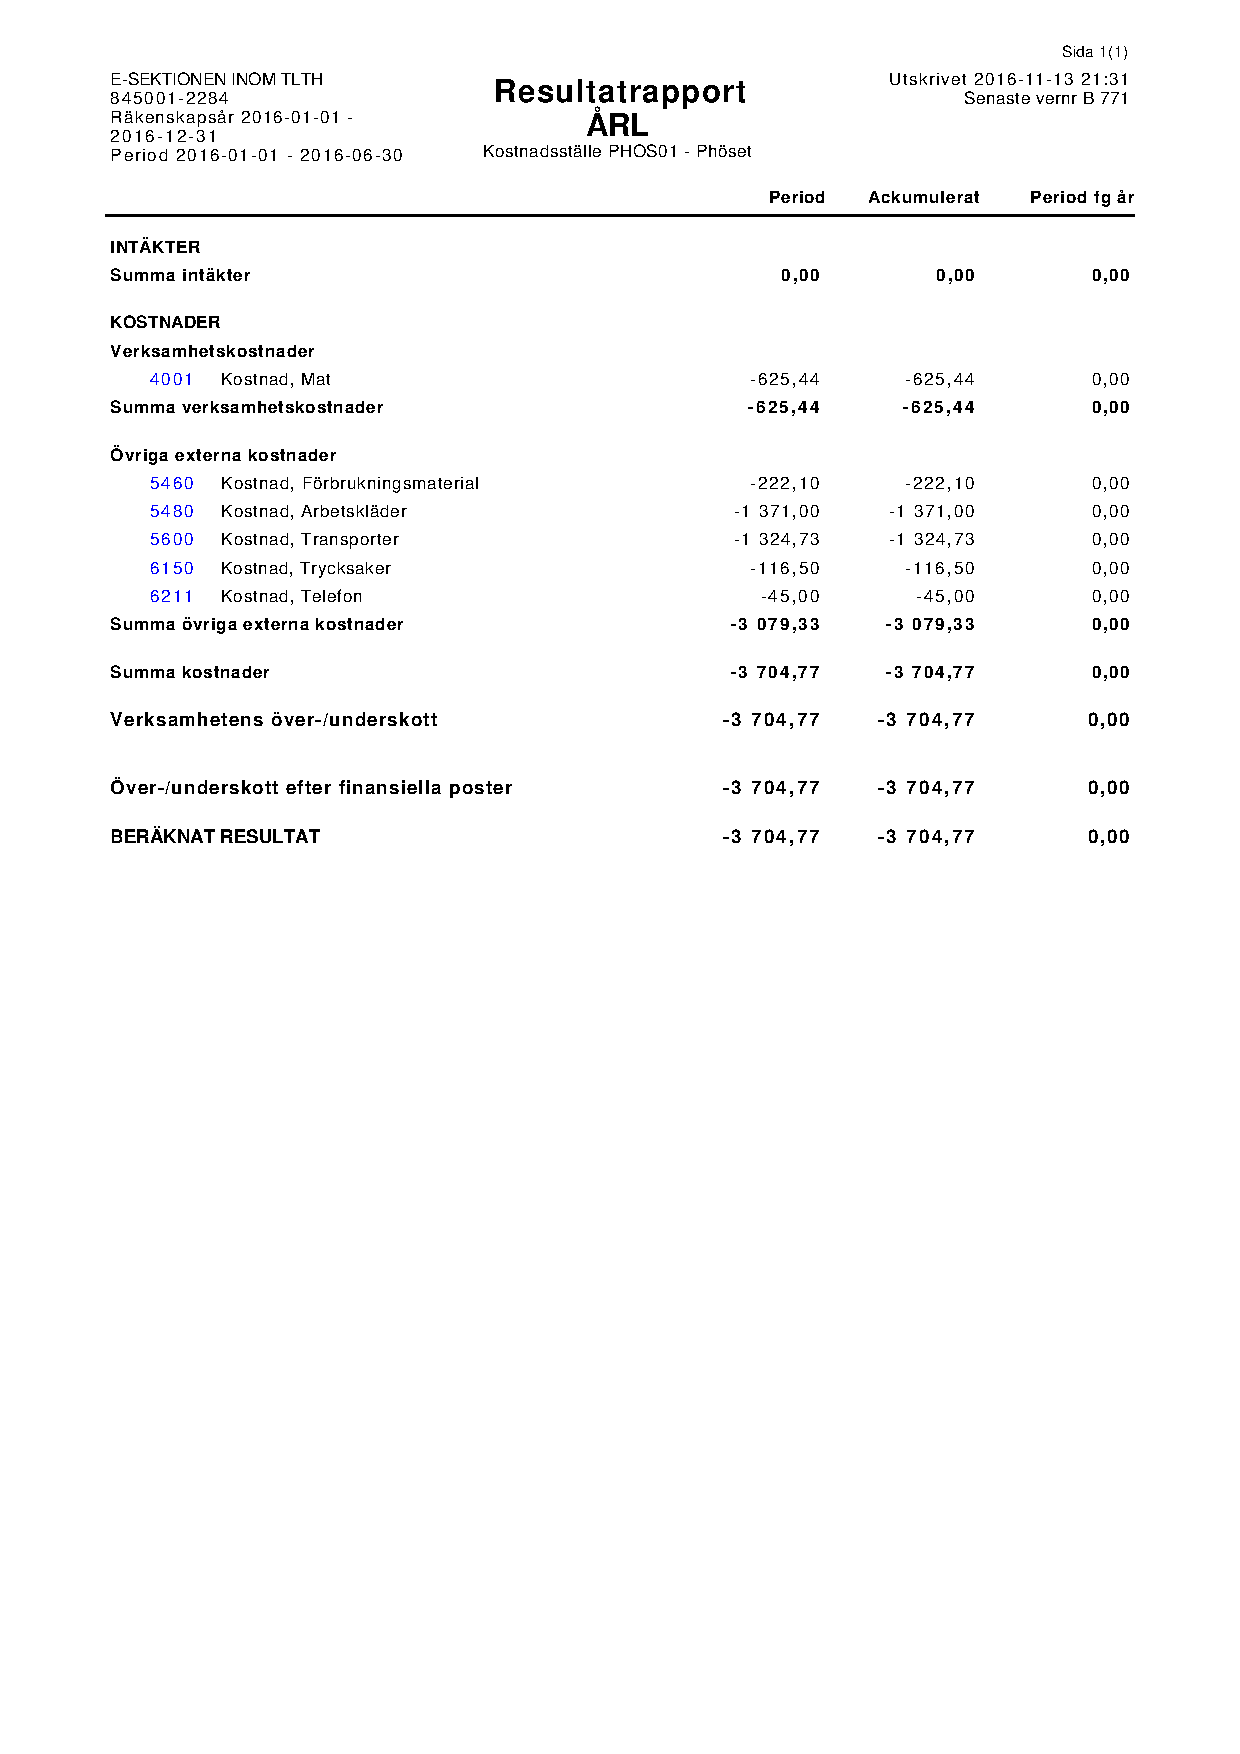
\includepdf[pages=-]{../_res/bokslut/phos01.pdf}
    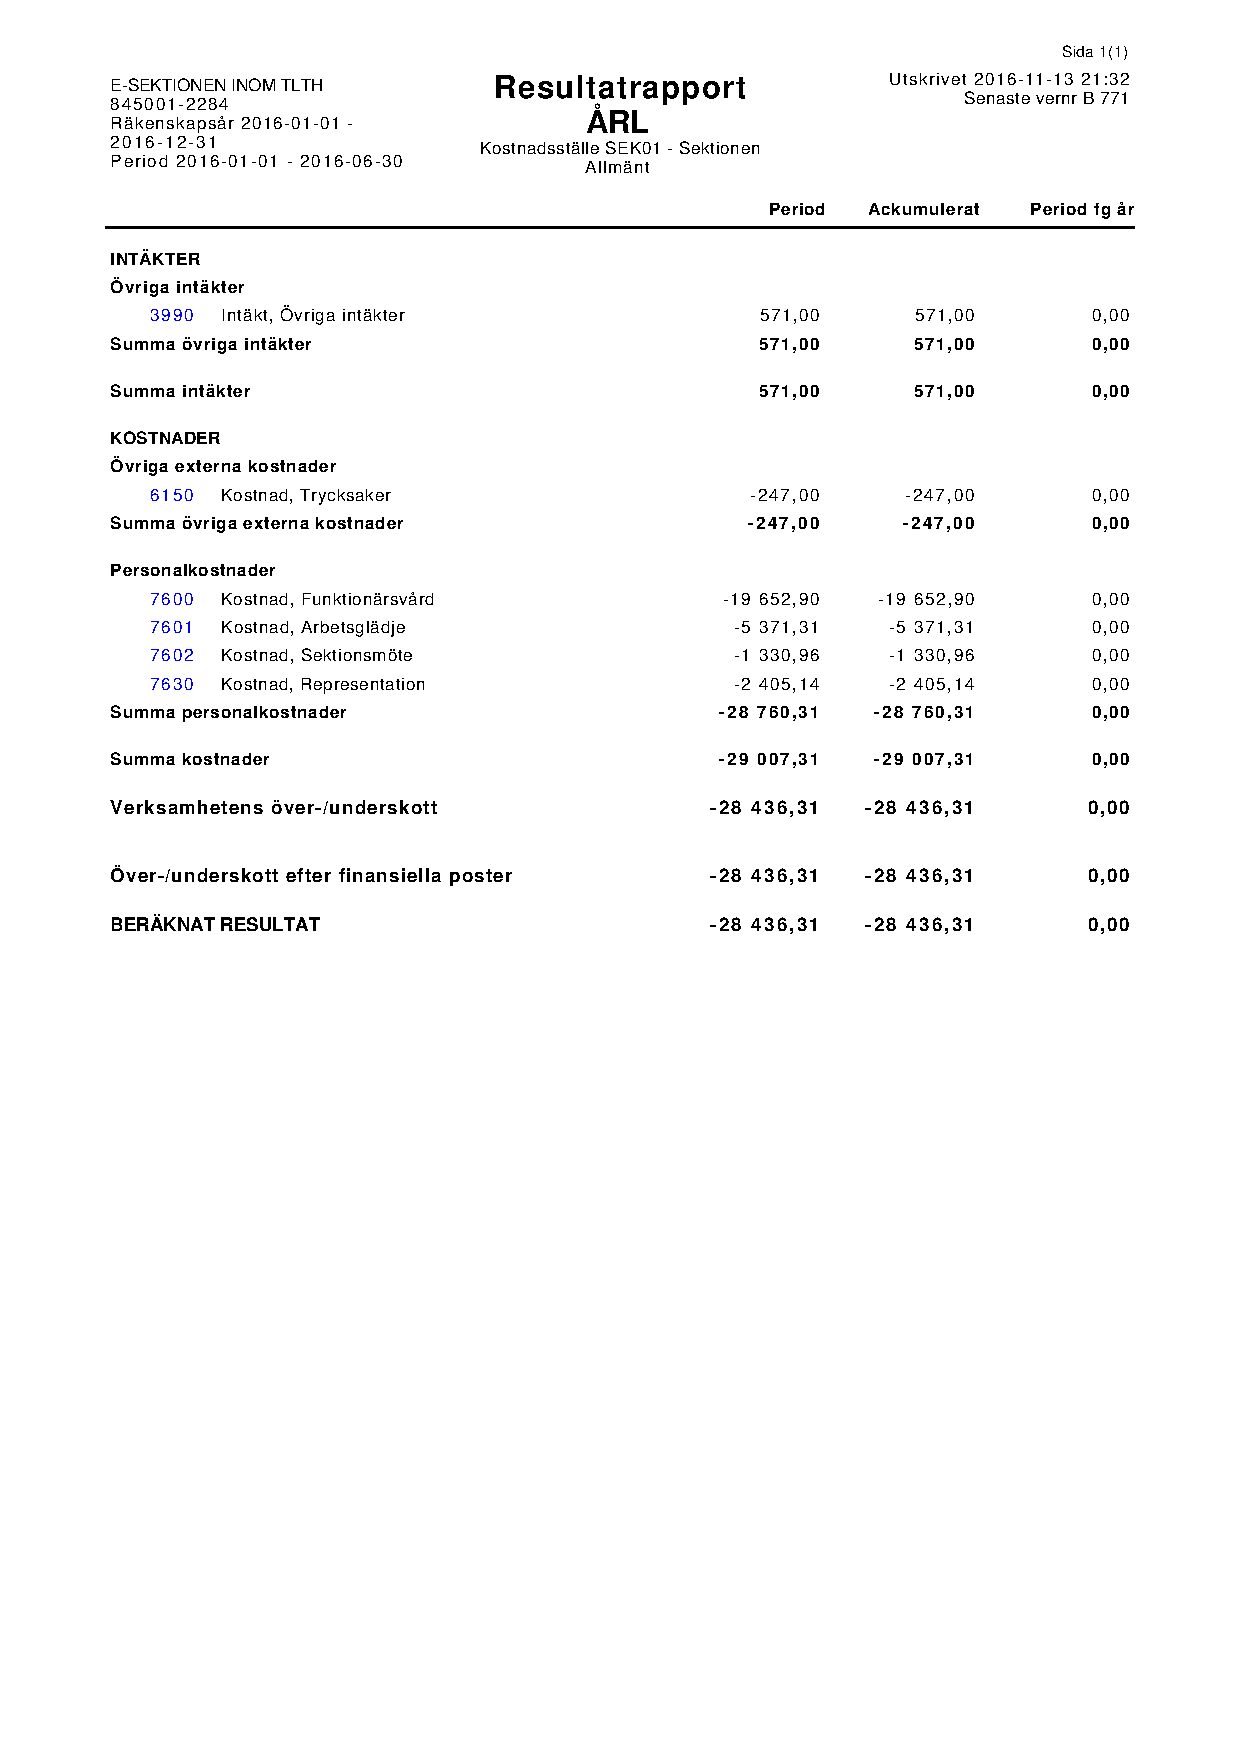
\includepdf[pages=-]{../_res/bokslut/sek01.pdf}
    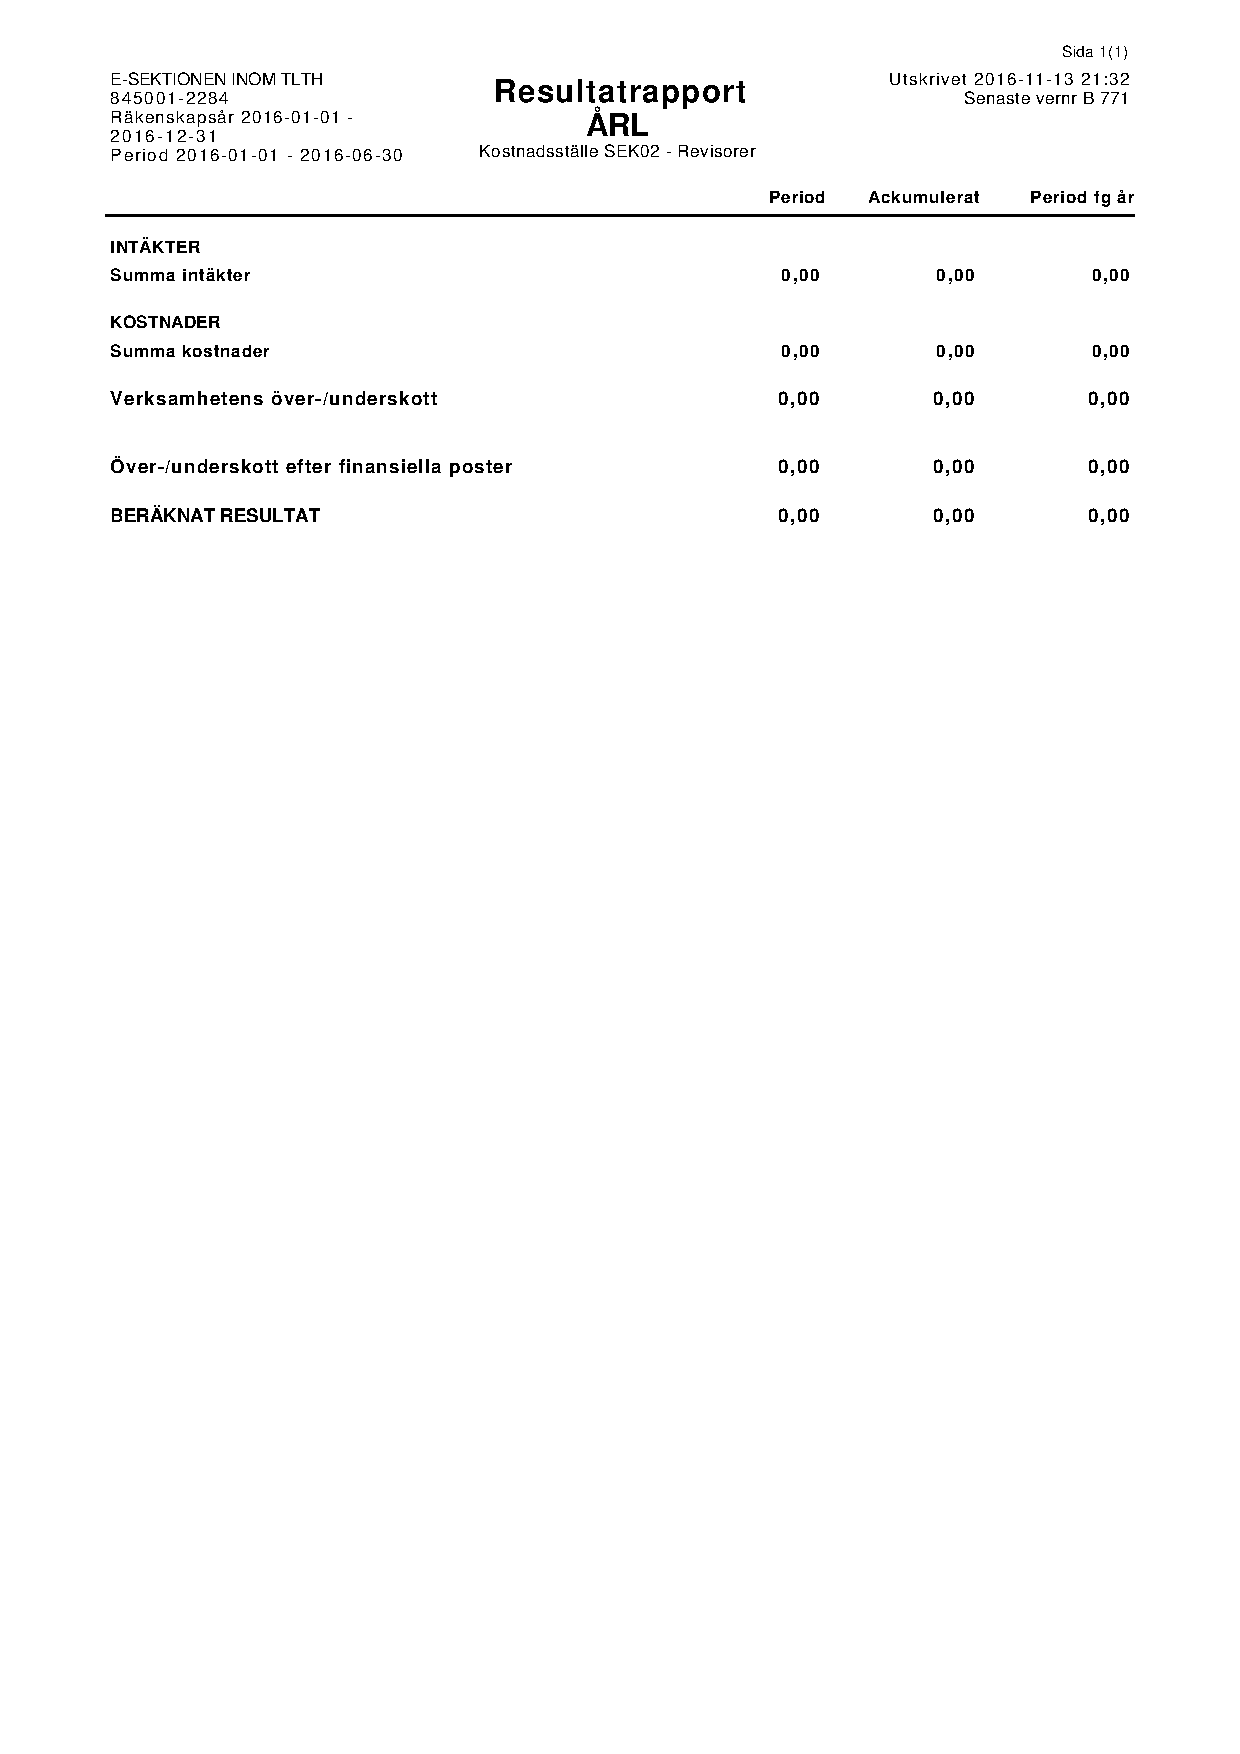
\includepdf[pages=-]{../_res/bokslut/sek02.pdf}
    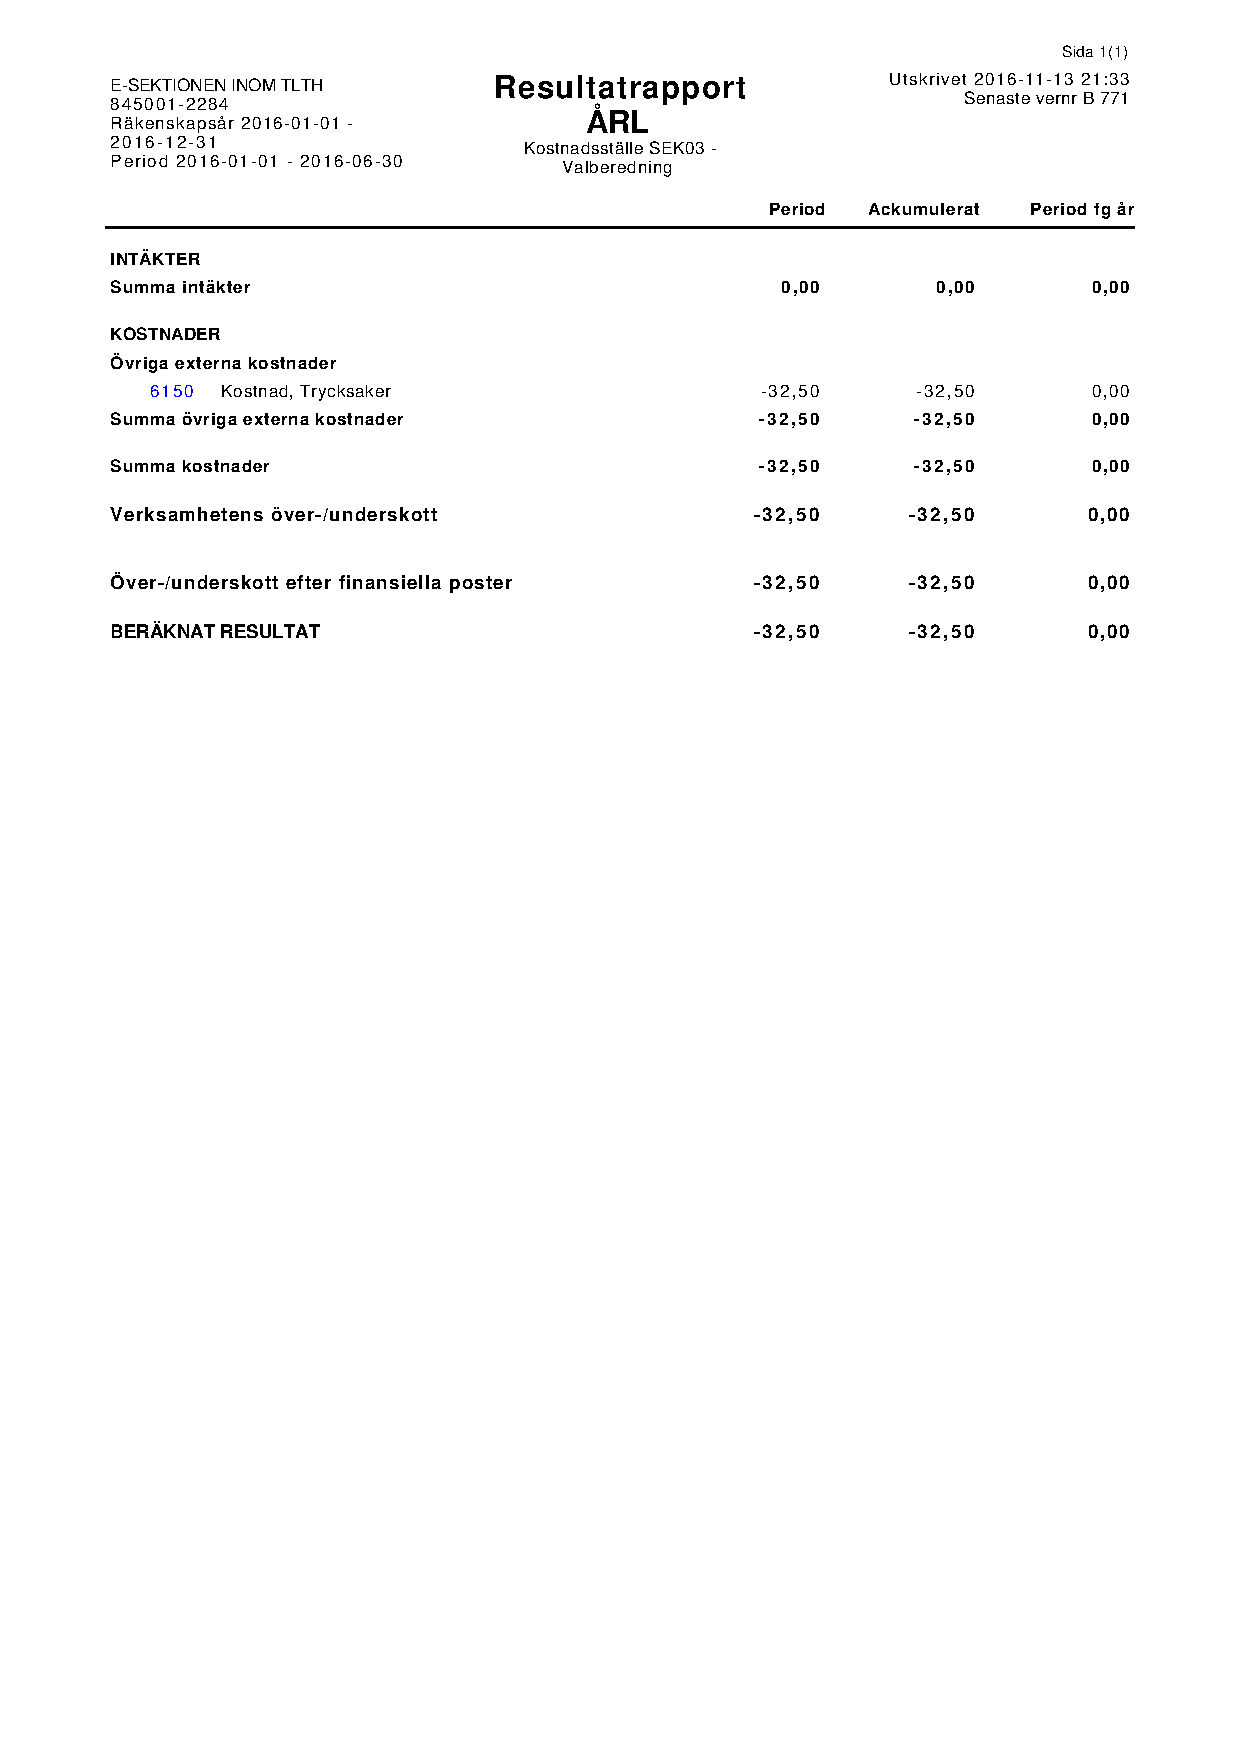
\includepdf[pages=-]{../_res/bokslut/sek04.pdf}
    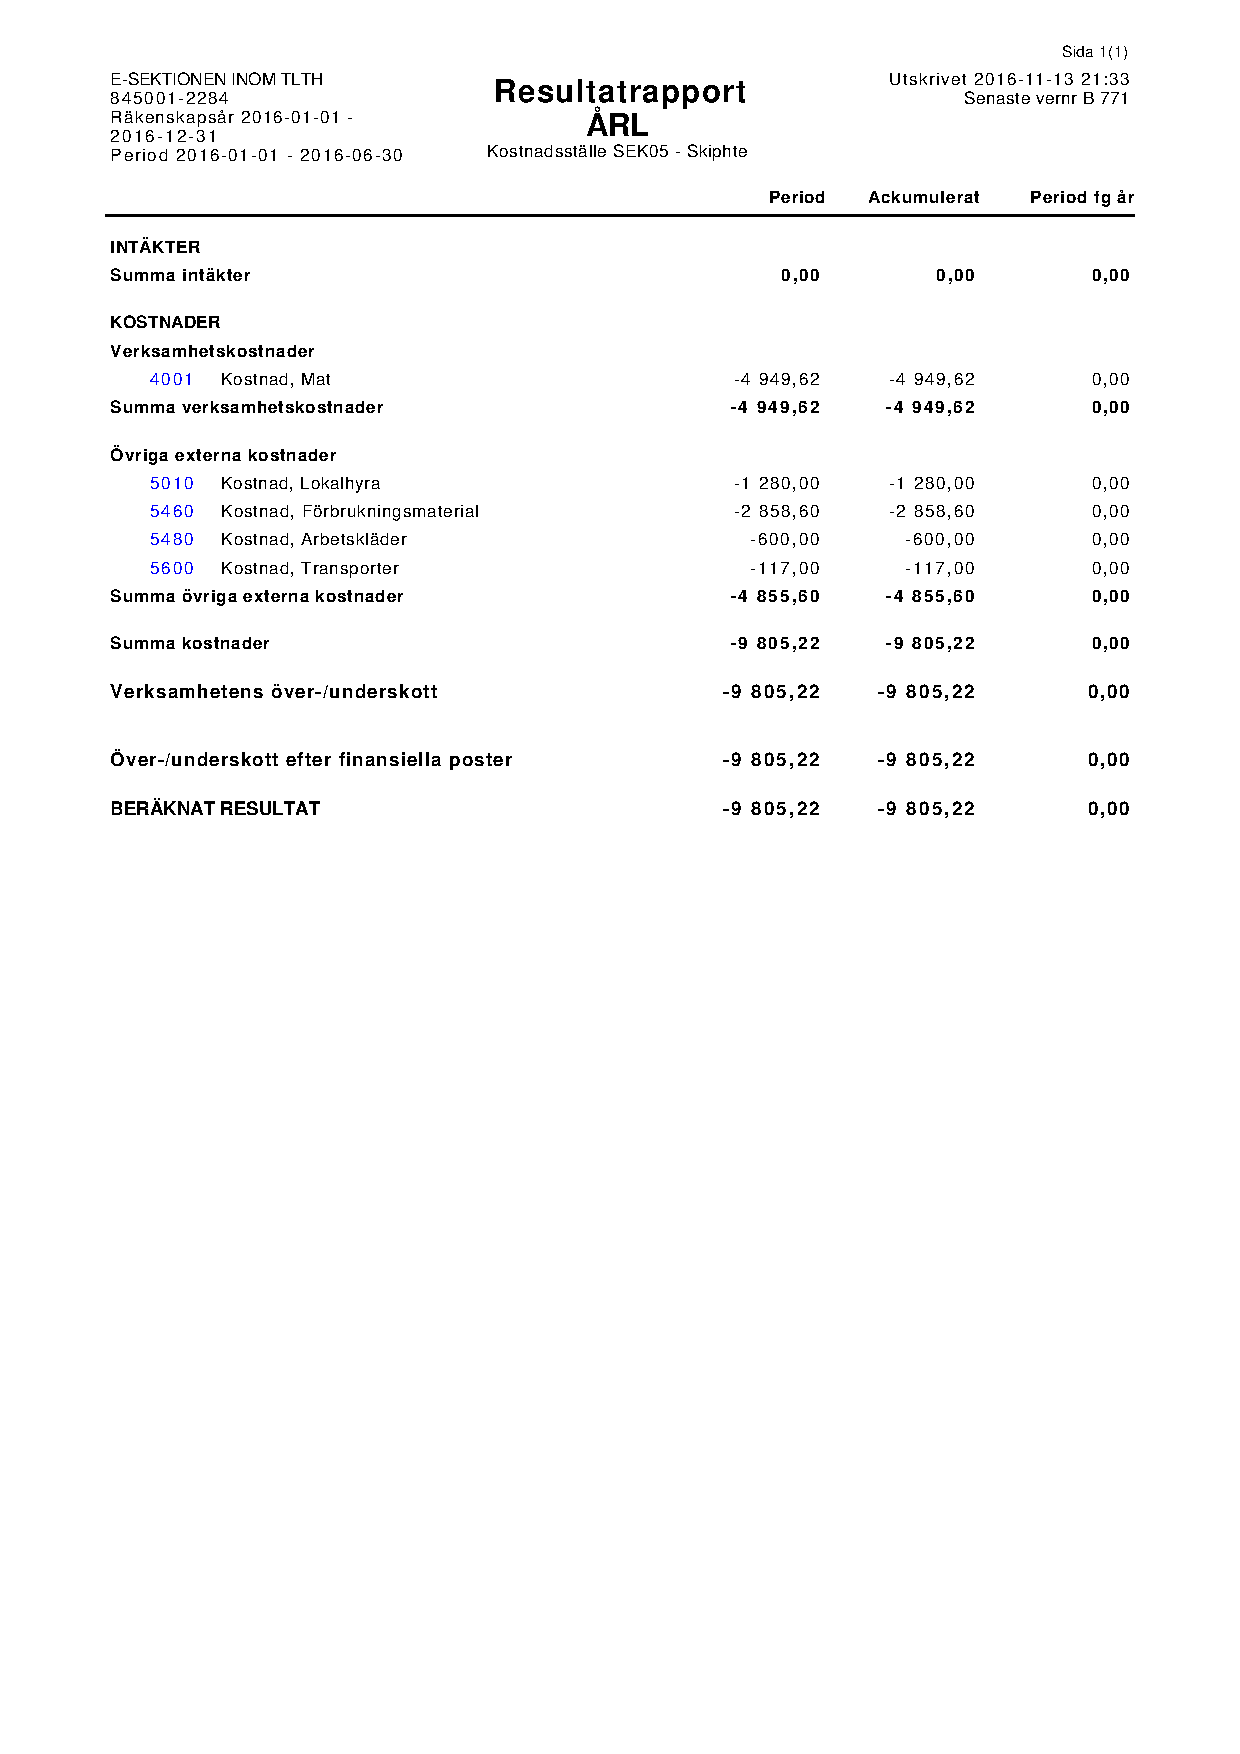
\includepdf[pages=-]{../_res/bokslut/sek05.pdf}
    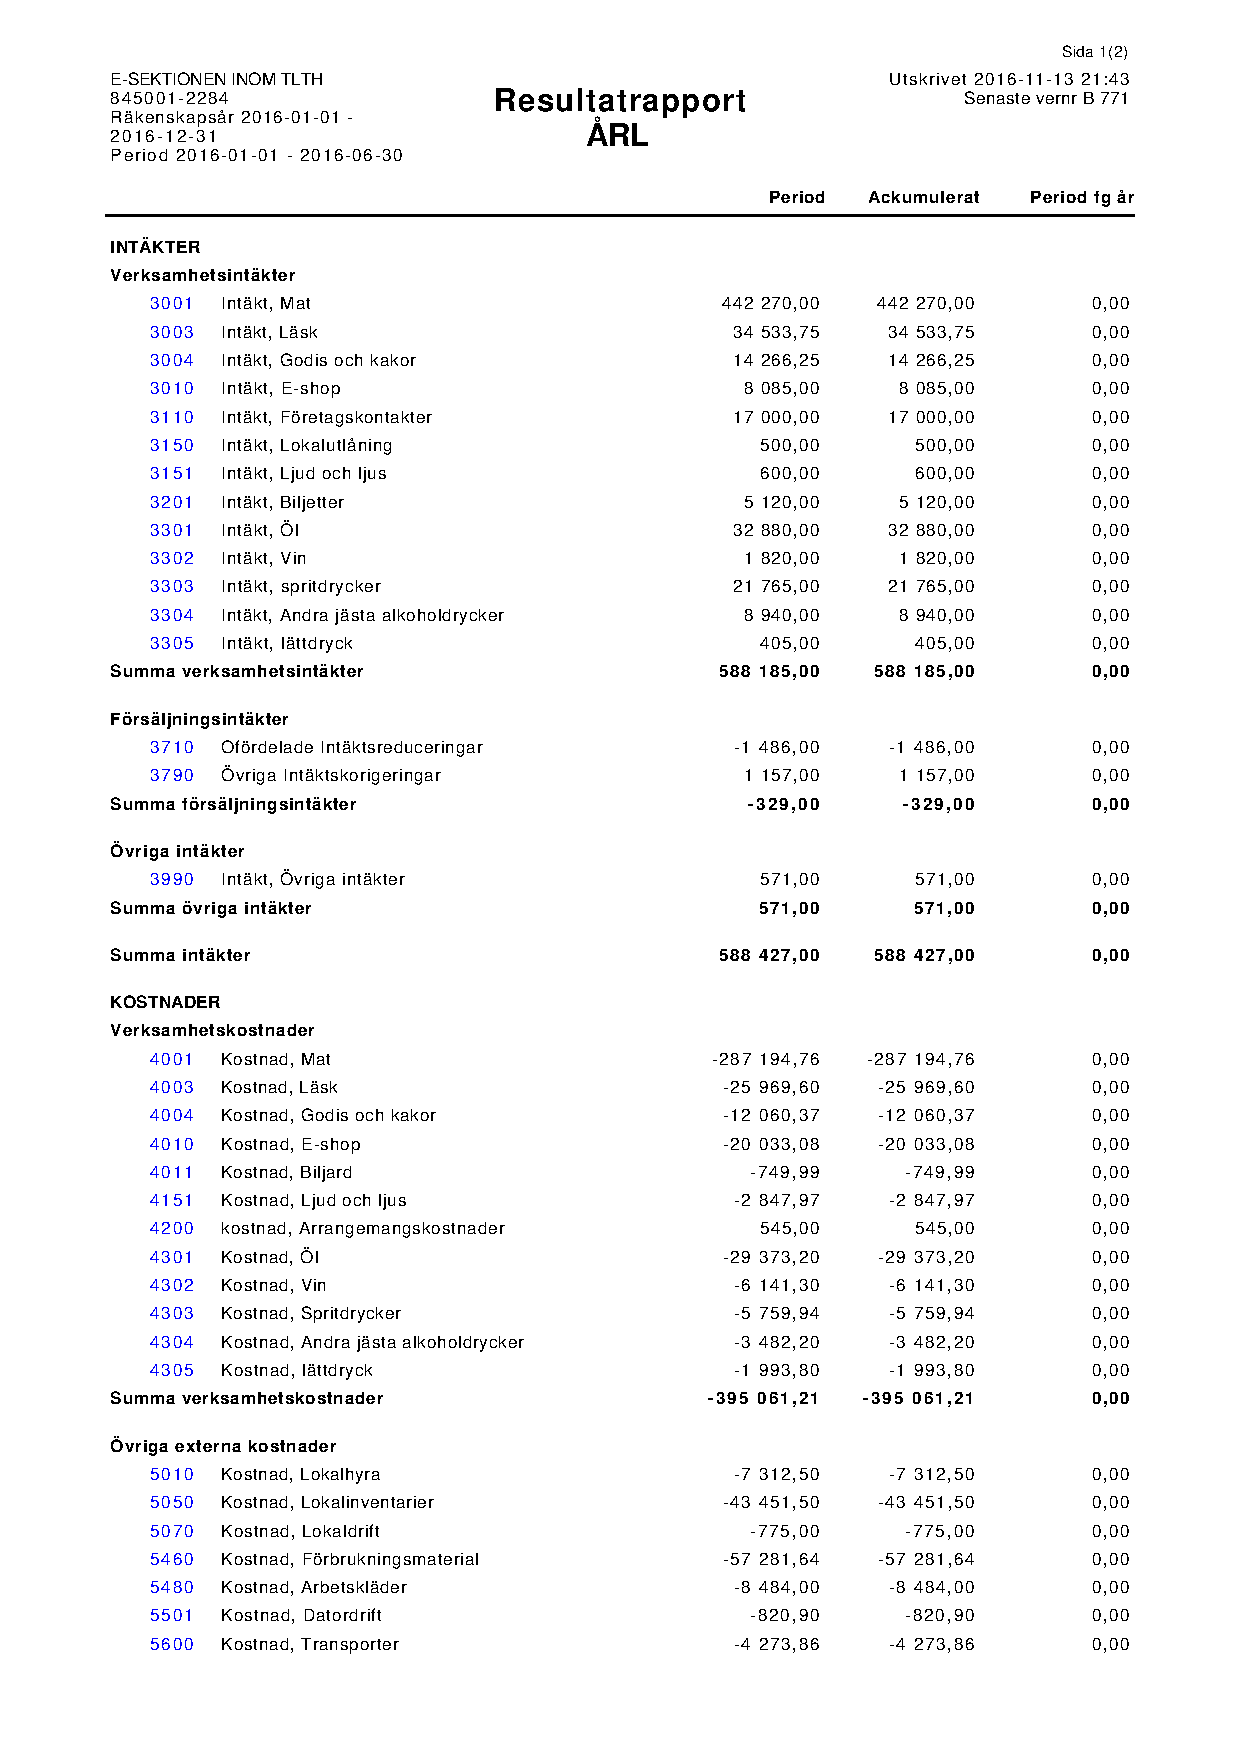
\includepdf[pages=-]{../_res/bokslut/sektionen.pdf}
    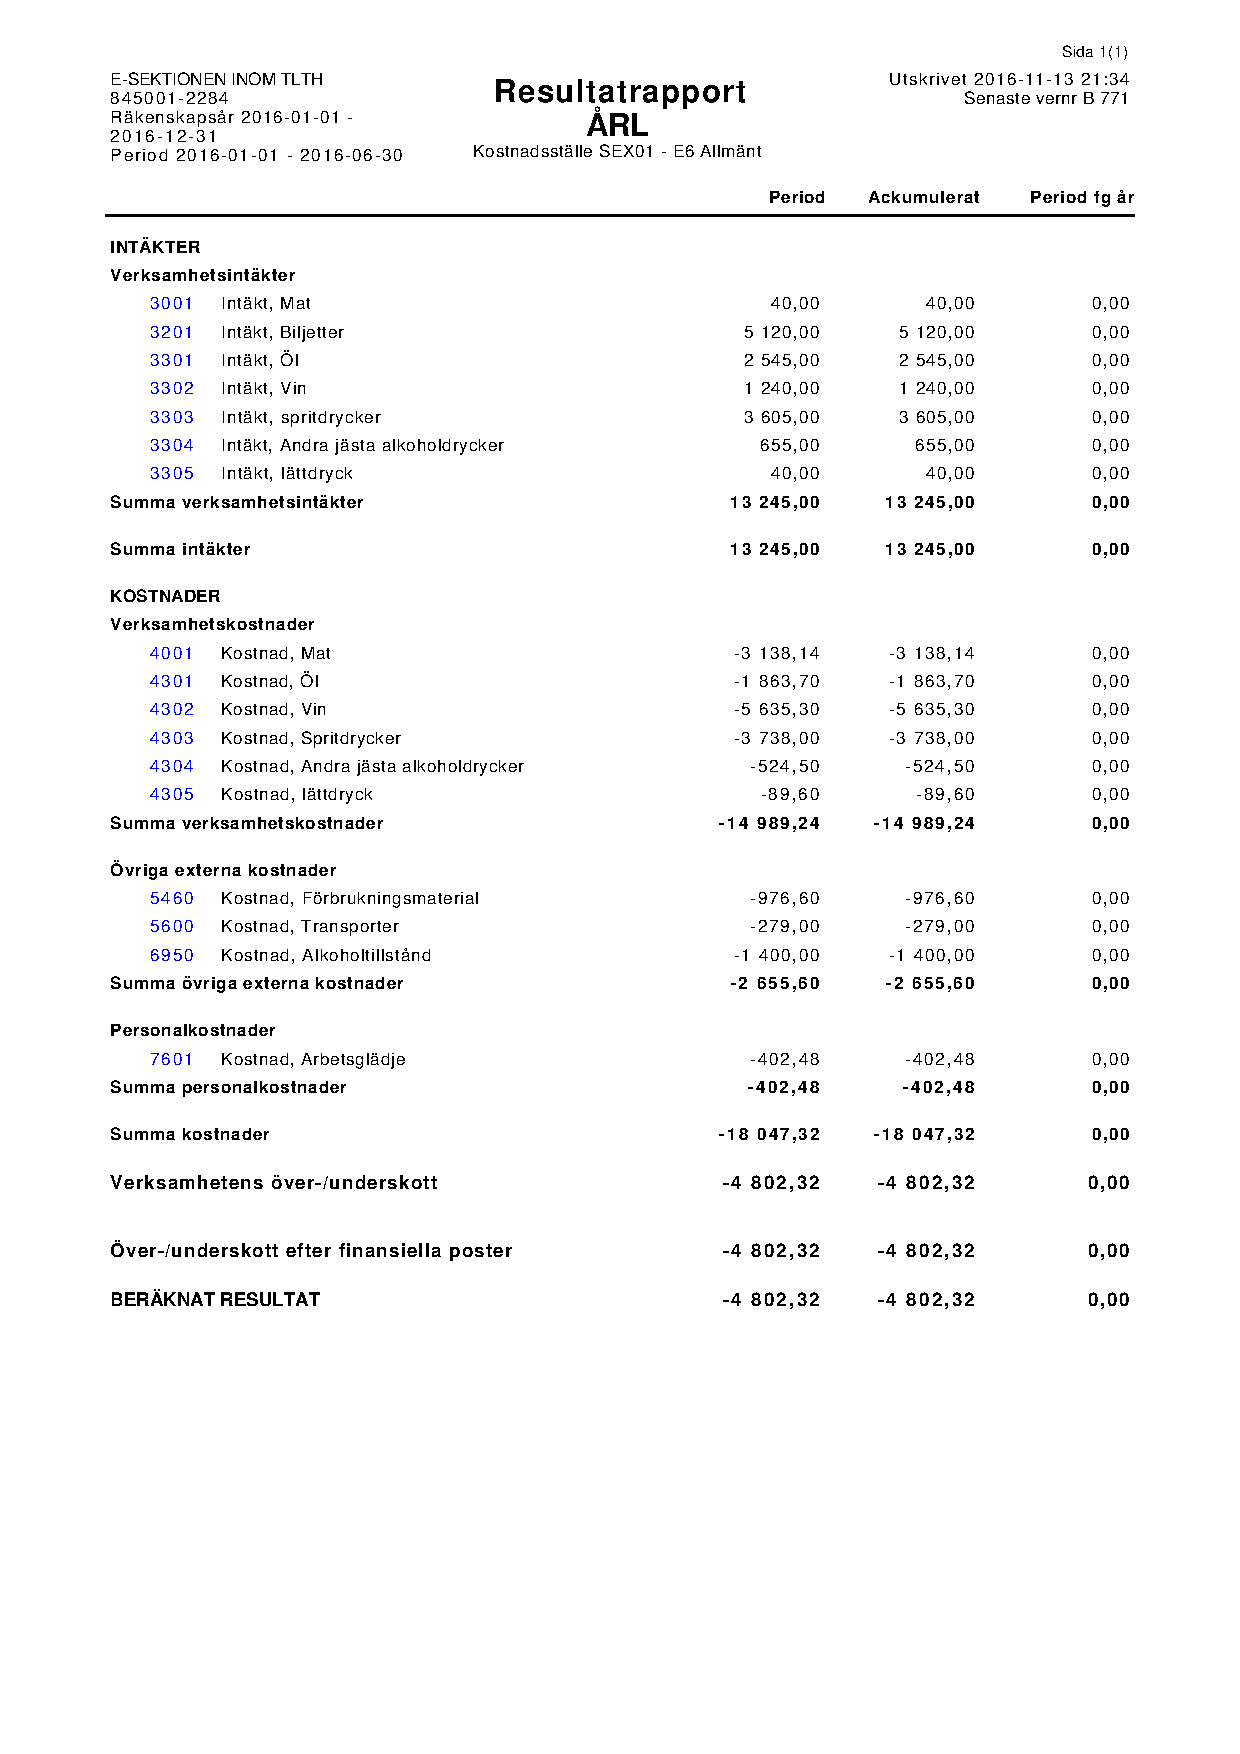
\includepdf[pages=-]{../_res/bokslut/sex01.pdf}
    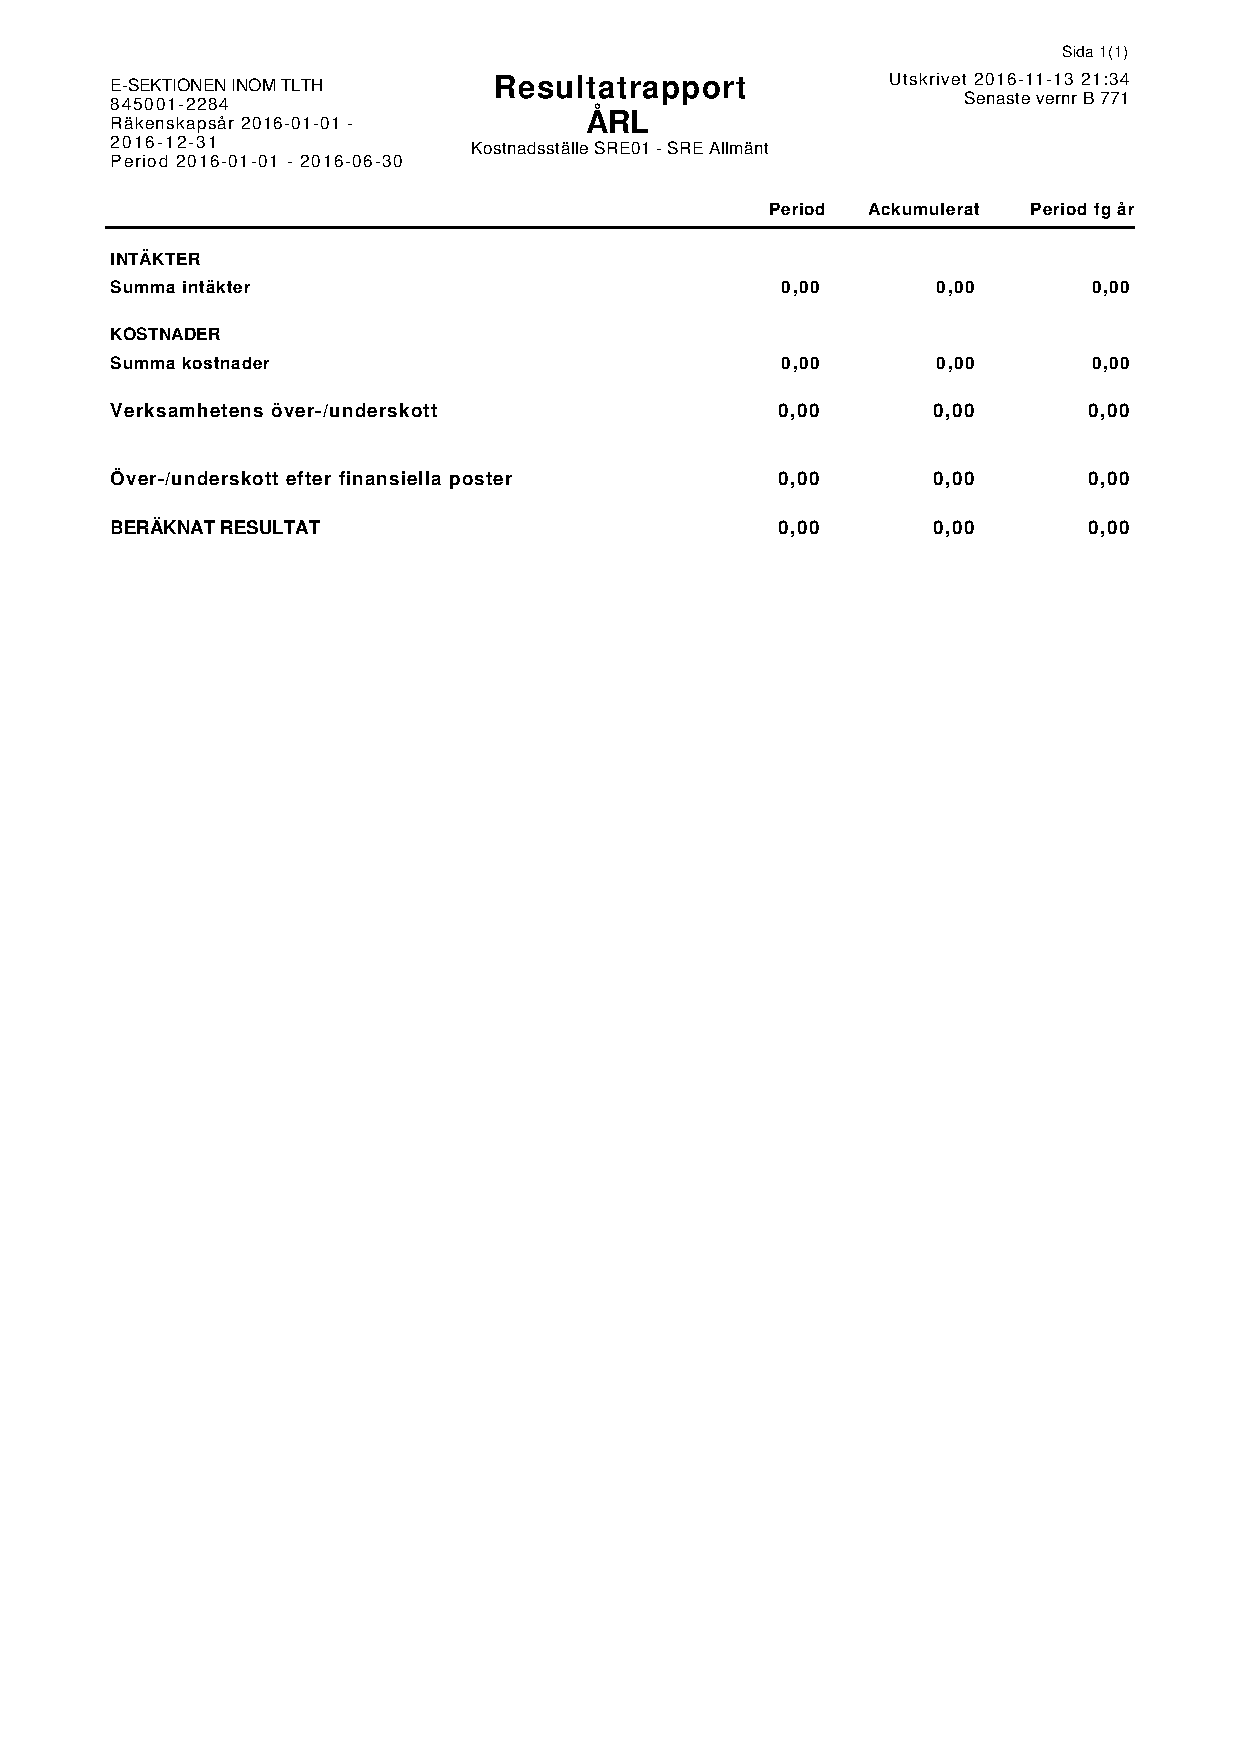
\includepdf[pages=-]{../_res/bokslut/sre01.pdf}
    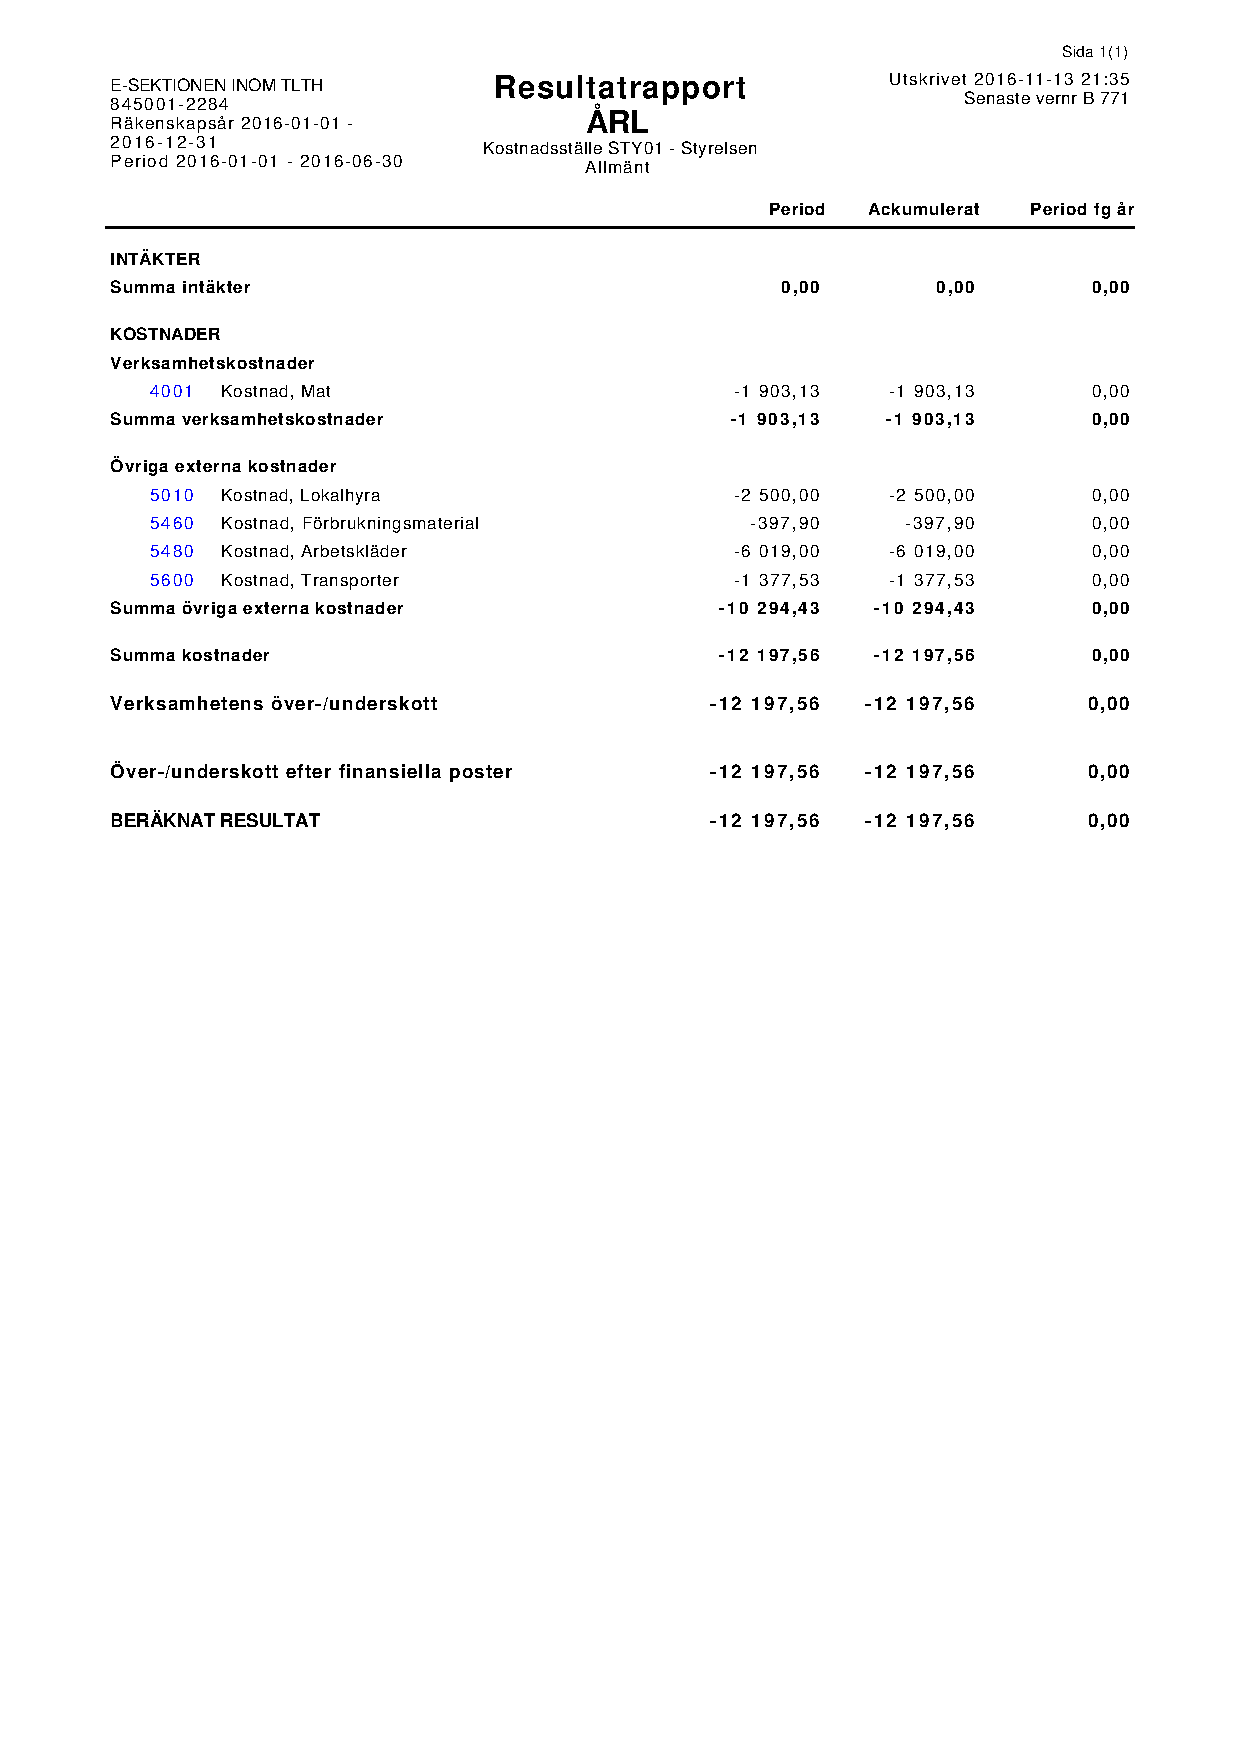
\includepdf[pages=-]{../_res/bokslut/sty01.pdf}
\end{supersection}

\end{document}
